\chapter{Results}
\label{chapter:Results}

\begin{introduction}
    "It always seems impossible until it's done." - Nelson Mandela, former President of South Africa
\end{introduction}

\section{Evolution of Software Development}

The software development process has undergone several important stages, each enhancing its functionality and usability. The figures below illustrate the application's progress, showcasing different phases of refinement as the project matured.

\subsection{Initial Stages: Basic Functionality and User Interaction}

The first figure (Figure \ref{fig:v1}) represents the early stages of development, where the primary focus was on creating a user-friendly interface for calculating Average Read Depth and Depth of Coverage at diferent threshold from a \ac{bam} file for a Single Gene. In this version, the application prominently features a two-step process where the user selects a \ac{bed} file releated to the gene to analyse and one or more \ac{bam} files. These files are then processed to calculate key metrics, which are displayed in a results table. This simple design allowed for efficient user interaction but was somewhat limited in terms of flexibility and scope.

At this stage, the core challenge was to ensure that the software could handle large genomic files while presenting the results in a clear and intuitive format. The layout emphasizes simplicity, making it easier for users to navigate through the two-step process. However, as the project progressed, the need for more advanced features became evident.

\begin{figure}[H]
    \centering
    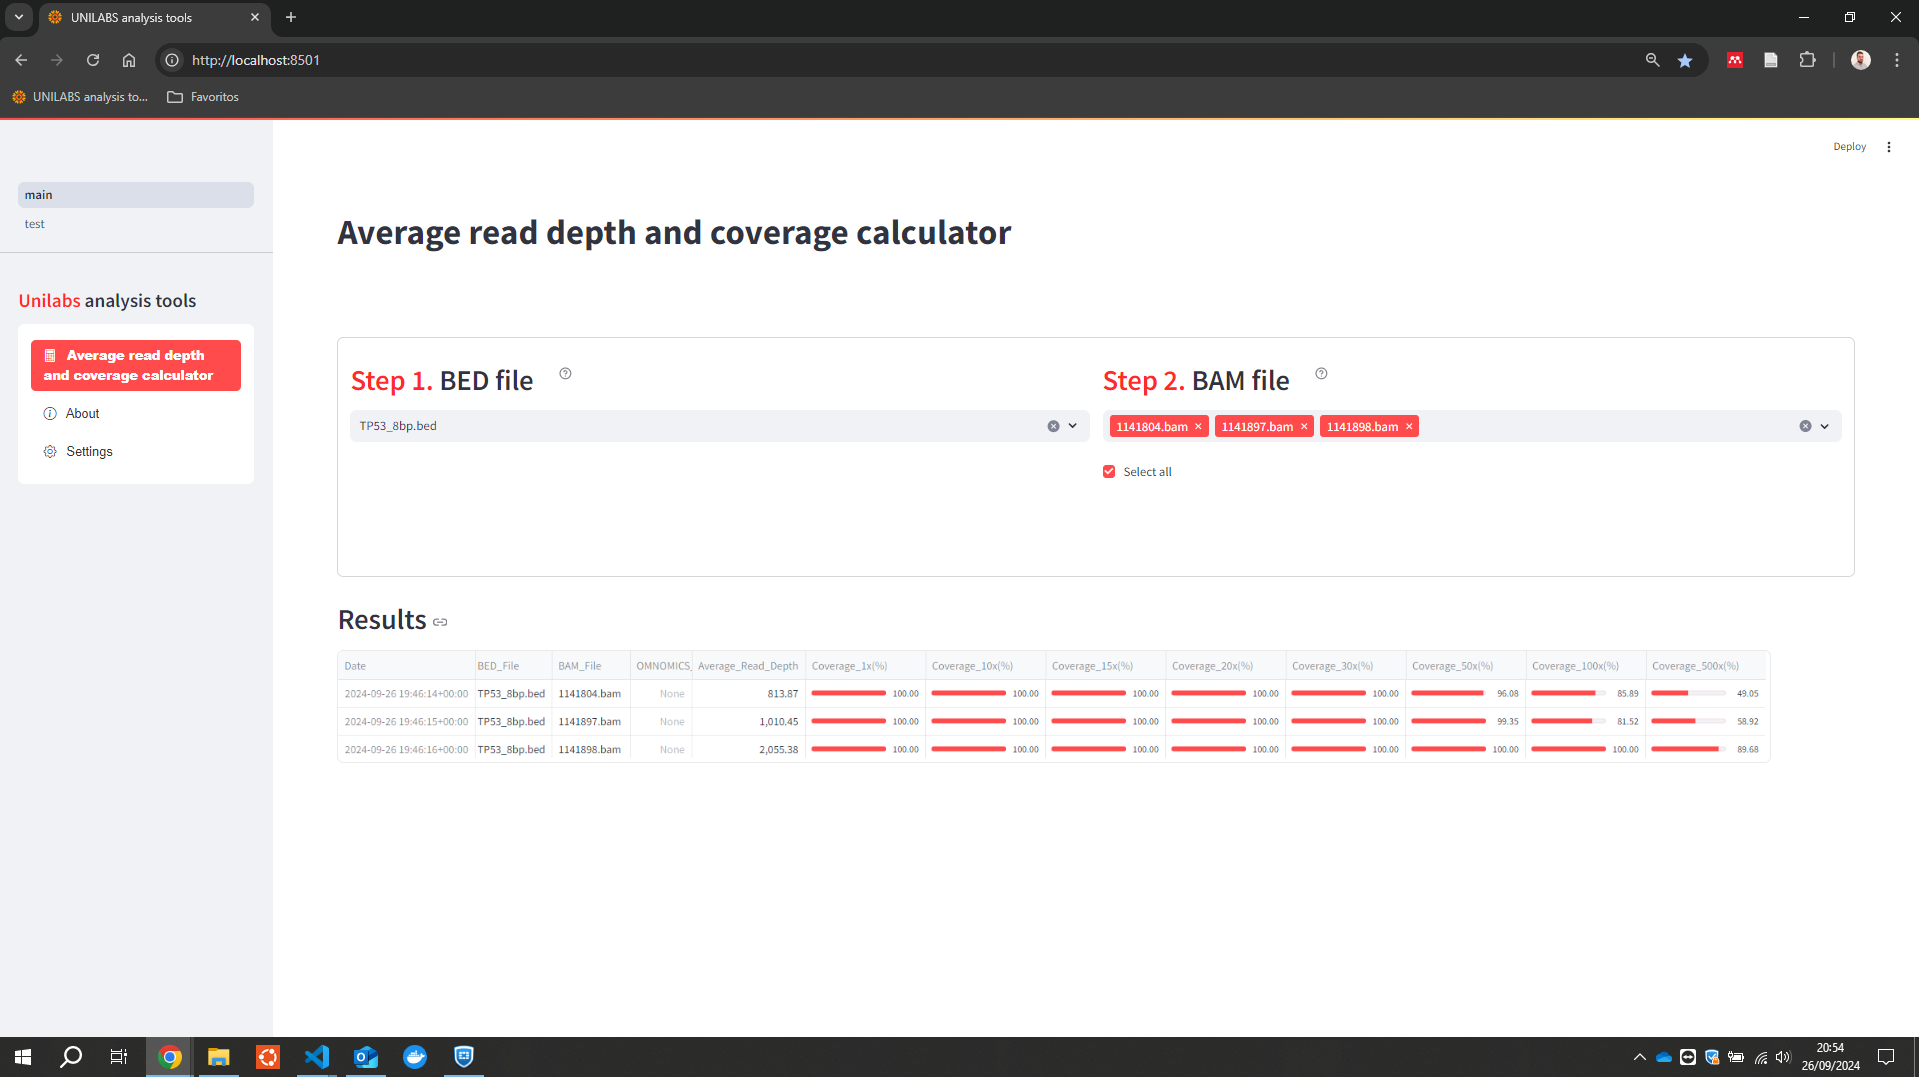
\includegraphics[width=1\textwidth]{figs/v1.png}
    \caption{First version of the \ac{gui}.} 
    \label{fig:v1}
\end{figure}

\subsection{Refinement: Introducing Flexibility and Multiple Analysis Modes}

In the second figure (Figure \ref{fig:v2}), the software has significantly evolved to include more detailed analysis options. The interface now presents multiple analysis types: \textit{Single Gene}, \textit{Gene Panel}, and \textit{Exome}, catering to different research needs. This flexibility represents a major shift from the earlier version, as it now allows users to select specific genome assemblies and regions of interest by using an Universal \ac{bed} file. Additionally, the results section has been split into tabs such as \textit{Overview} and \textit{Exon Details}, giving users the ability to drill down into the metrics for a the gene or explore exon-level coverage details. However, even though this last features were thinked to be used in this version, they only have been work fully in the last version of the software.

\begin{figure}[H]
    \centering
    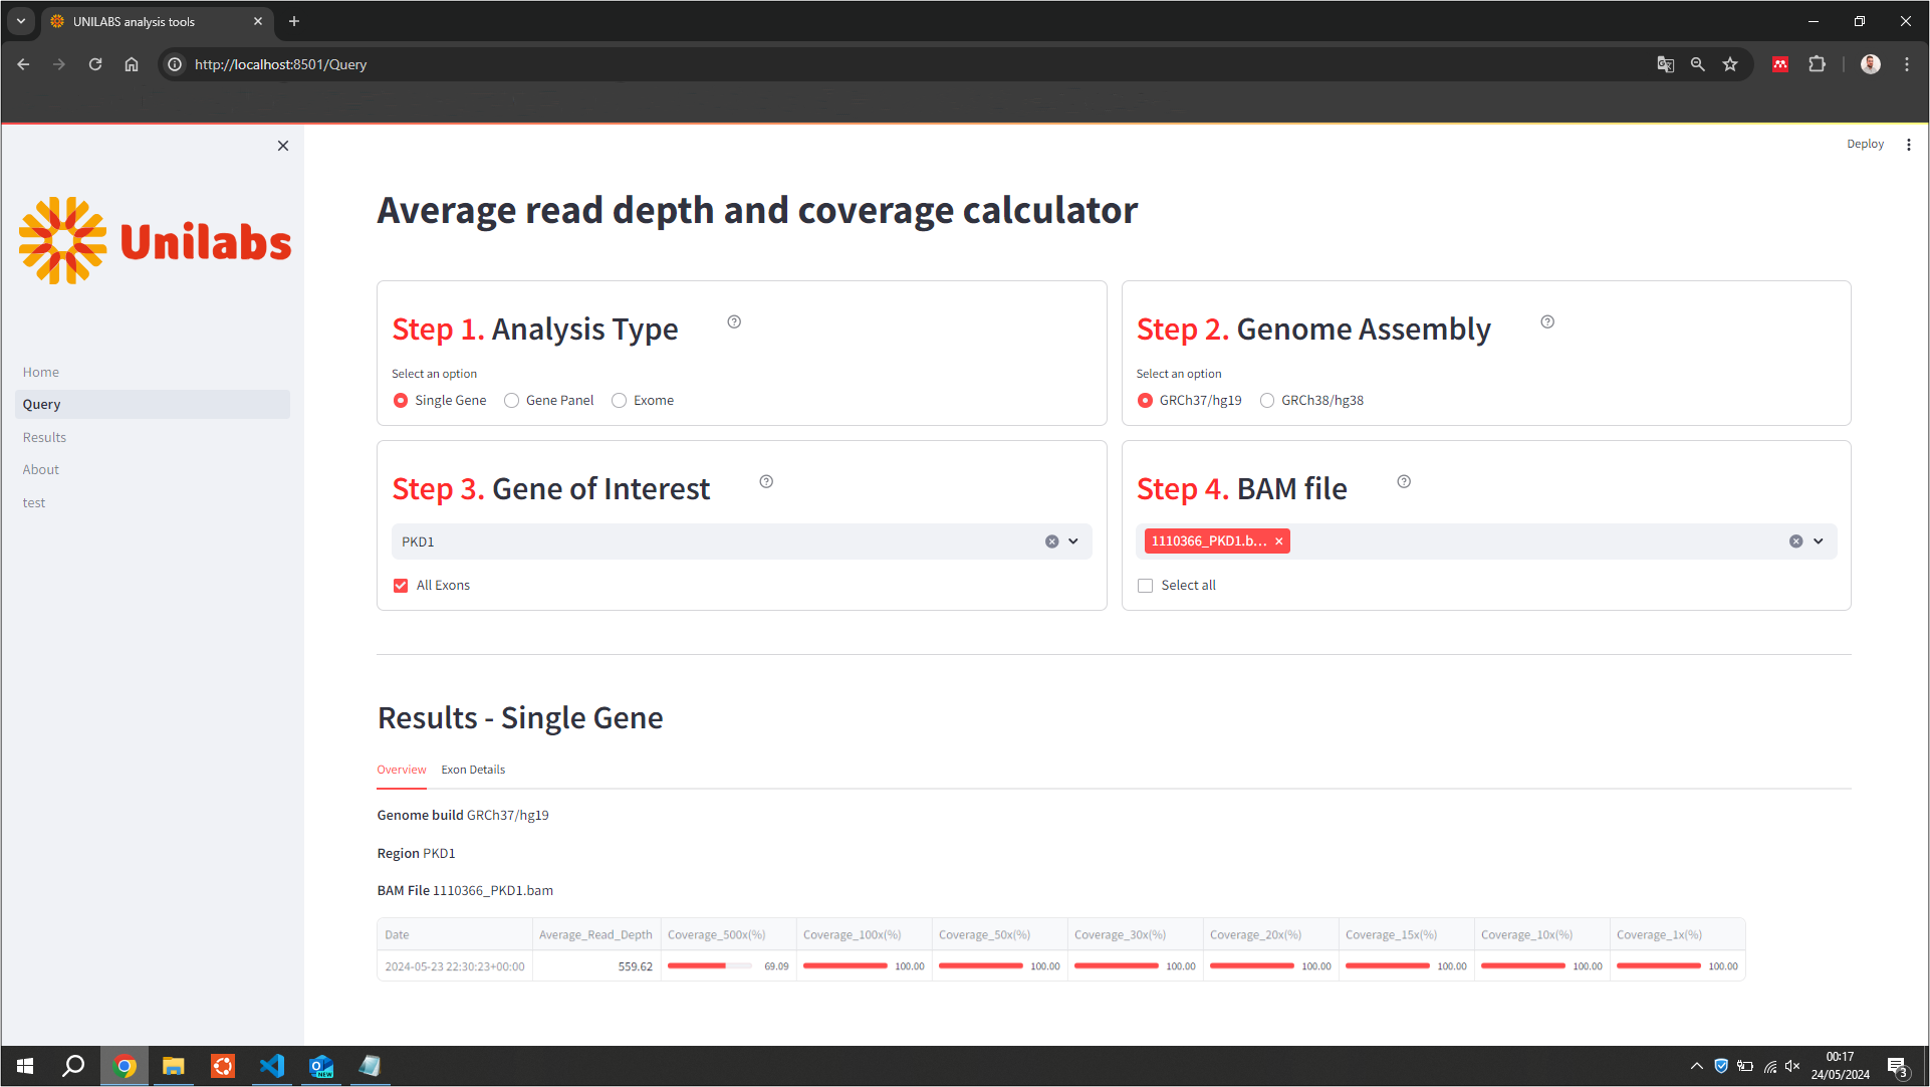
\includegraphics[width=1\textwidth]{figs/v2.png}
    \caption{Second version of the \ac{gui}.} 
    \label{fig:v2}
\end{figure}


The final version of the software is presented in the next section in detail with real-world data to showcase its full capabilities and effectiveness in genomic analysis. This final iteration represents the culmination of numerous improvements in both the user interface and the backend computational logic.

\subsection{Overview of the Final Version}

The final version of the software maintains the core functionality established in earlier versions, such as calculating Average Read Depth and Depth of Coverage from \ac{bed} and \ac{bam} files. However, it has evolved to include more refined features, enhanced performance, and the ability to handle more complex datasets.

This section presents a detailed overview of the final version of the software using real-world genomic data, illustrating its capabilities in calculating Depth and Breadth of Coverage for genomic regions of interest. The images provided demonstrate the final interface and processing stages.

\subsubsection{\textbf{Login Interface}}

As seen in Figure \ref{fig:login}, the software begins with a user authentication process, offering a simple and clean login interface. This feature, although optional in the final deployment, ensures that access to sensitive data is controlled. However, it is important to note that the current implementation of the login interface is a prototypical version and does not offer any form of security. The system does not perform encryption or validation of credentials beyond basic checks, and therefore it should not be relied upon for securing sensitive information. Further development would be required to implement a secure authentication system if needed in future deployments.

\begin{figure}[H]
    \centering
    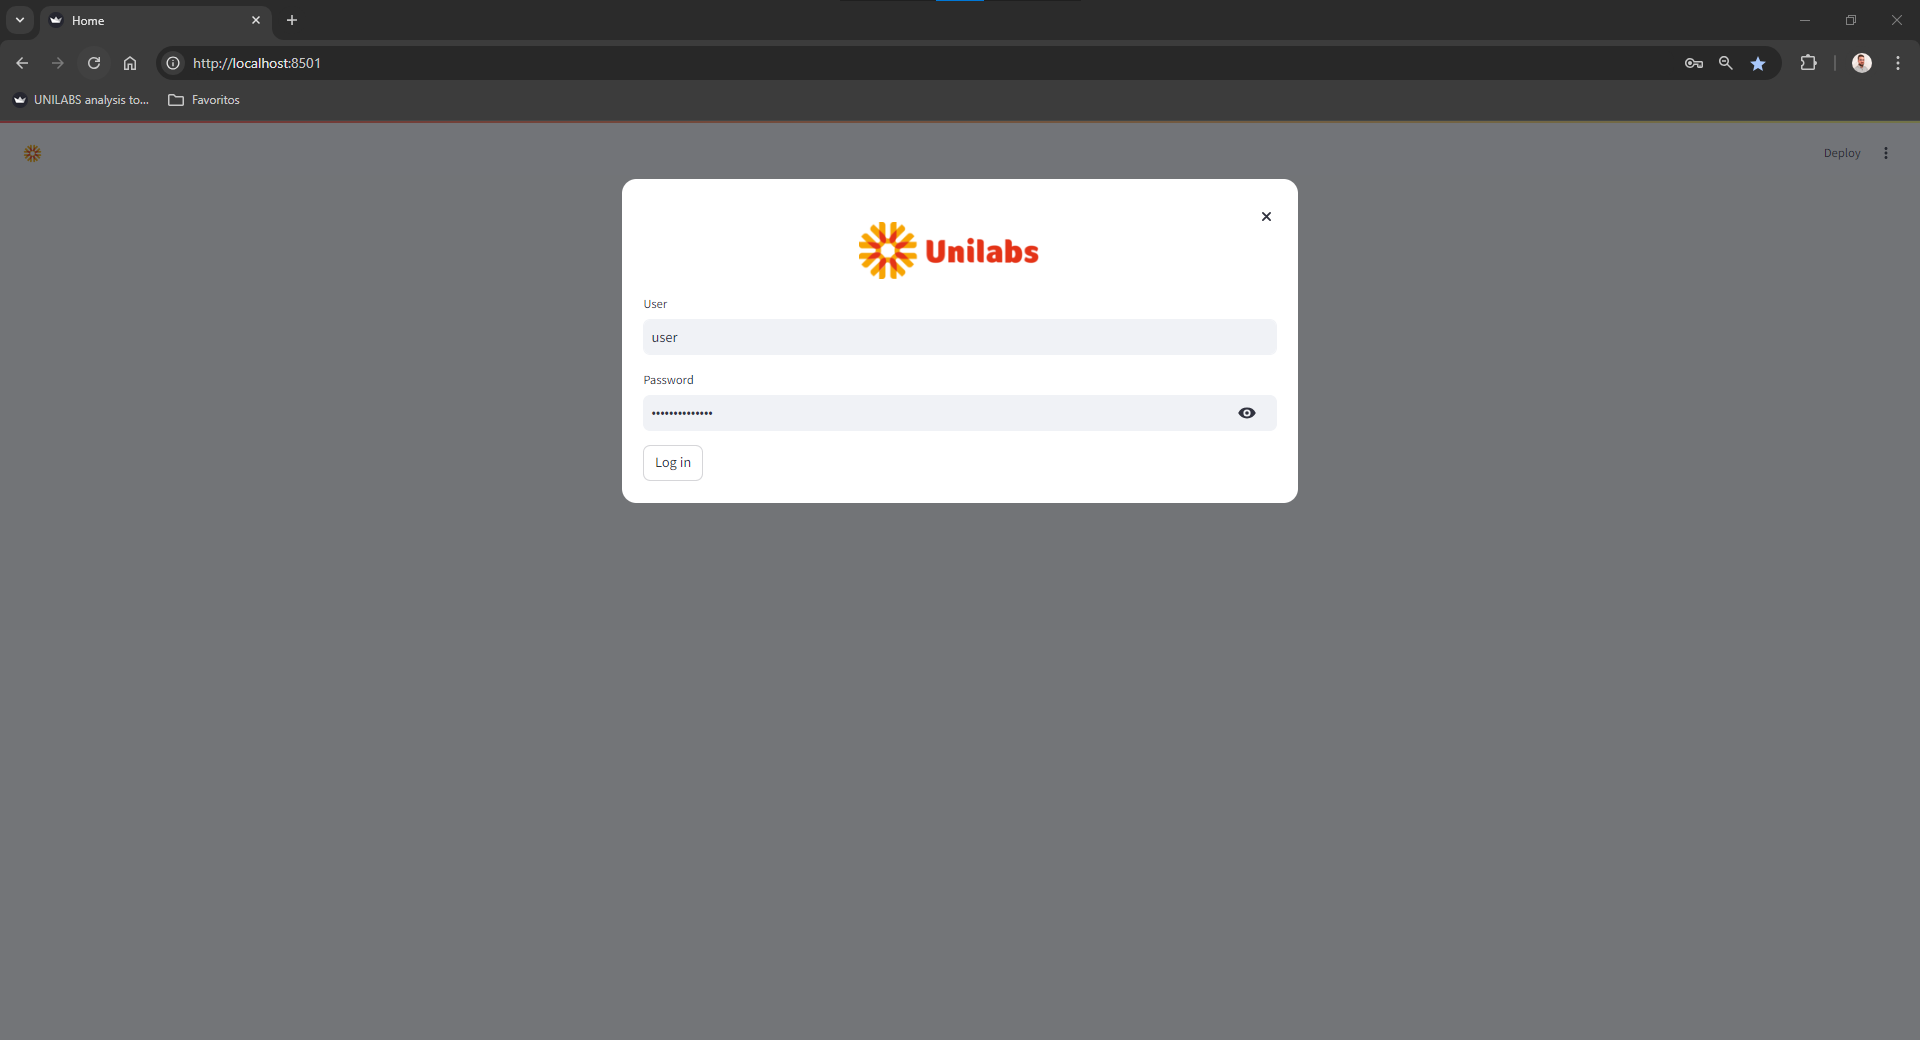
\includegraphics[width=\textwidth]{figs/v3.1.png}
    \caption{Login Interface for the Software}
    \label{fig:login}
\end{figure}

The next step of the process involves selecting the analysis type, as shown in Figure \ref{fig:single_gene}. Users can choose between three options: Single Gene, Gene Panel, and Exome. This selection determines the scope of the analysis and the subsequent steps in the workflow.


\subsubsection{\textbf{Single Gene Analysis}}

In this version, users can perform a single gene analysis by selecting the appropriate options for genome assembly and gene of interest. The software also provides the option to analyze all exons within the selected gene or focus on specific exons of interest. \ac{bam}/\ac{cram} files containing the sequencing data are acessed and processed by Samtools for detailed metrics.

\begin{figure}[H]
    \centering
    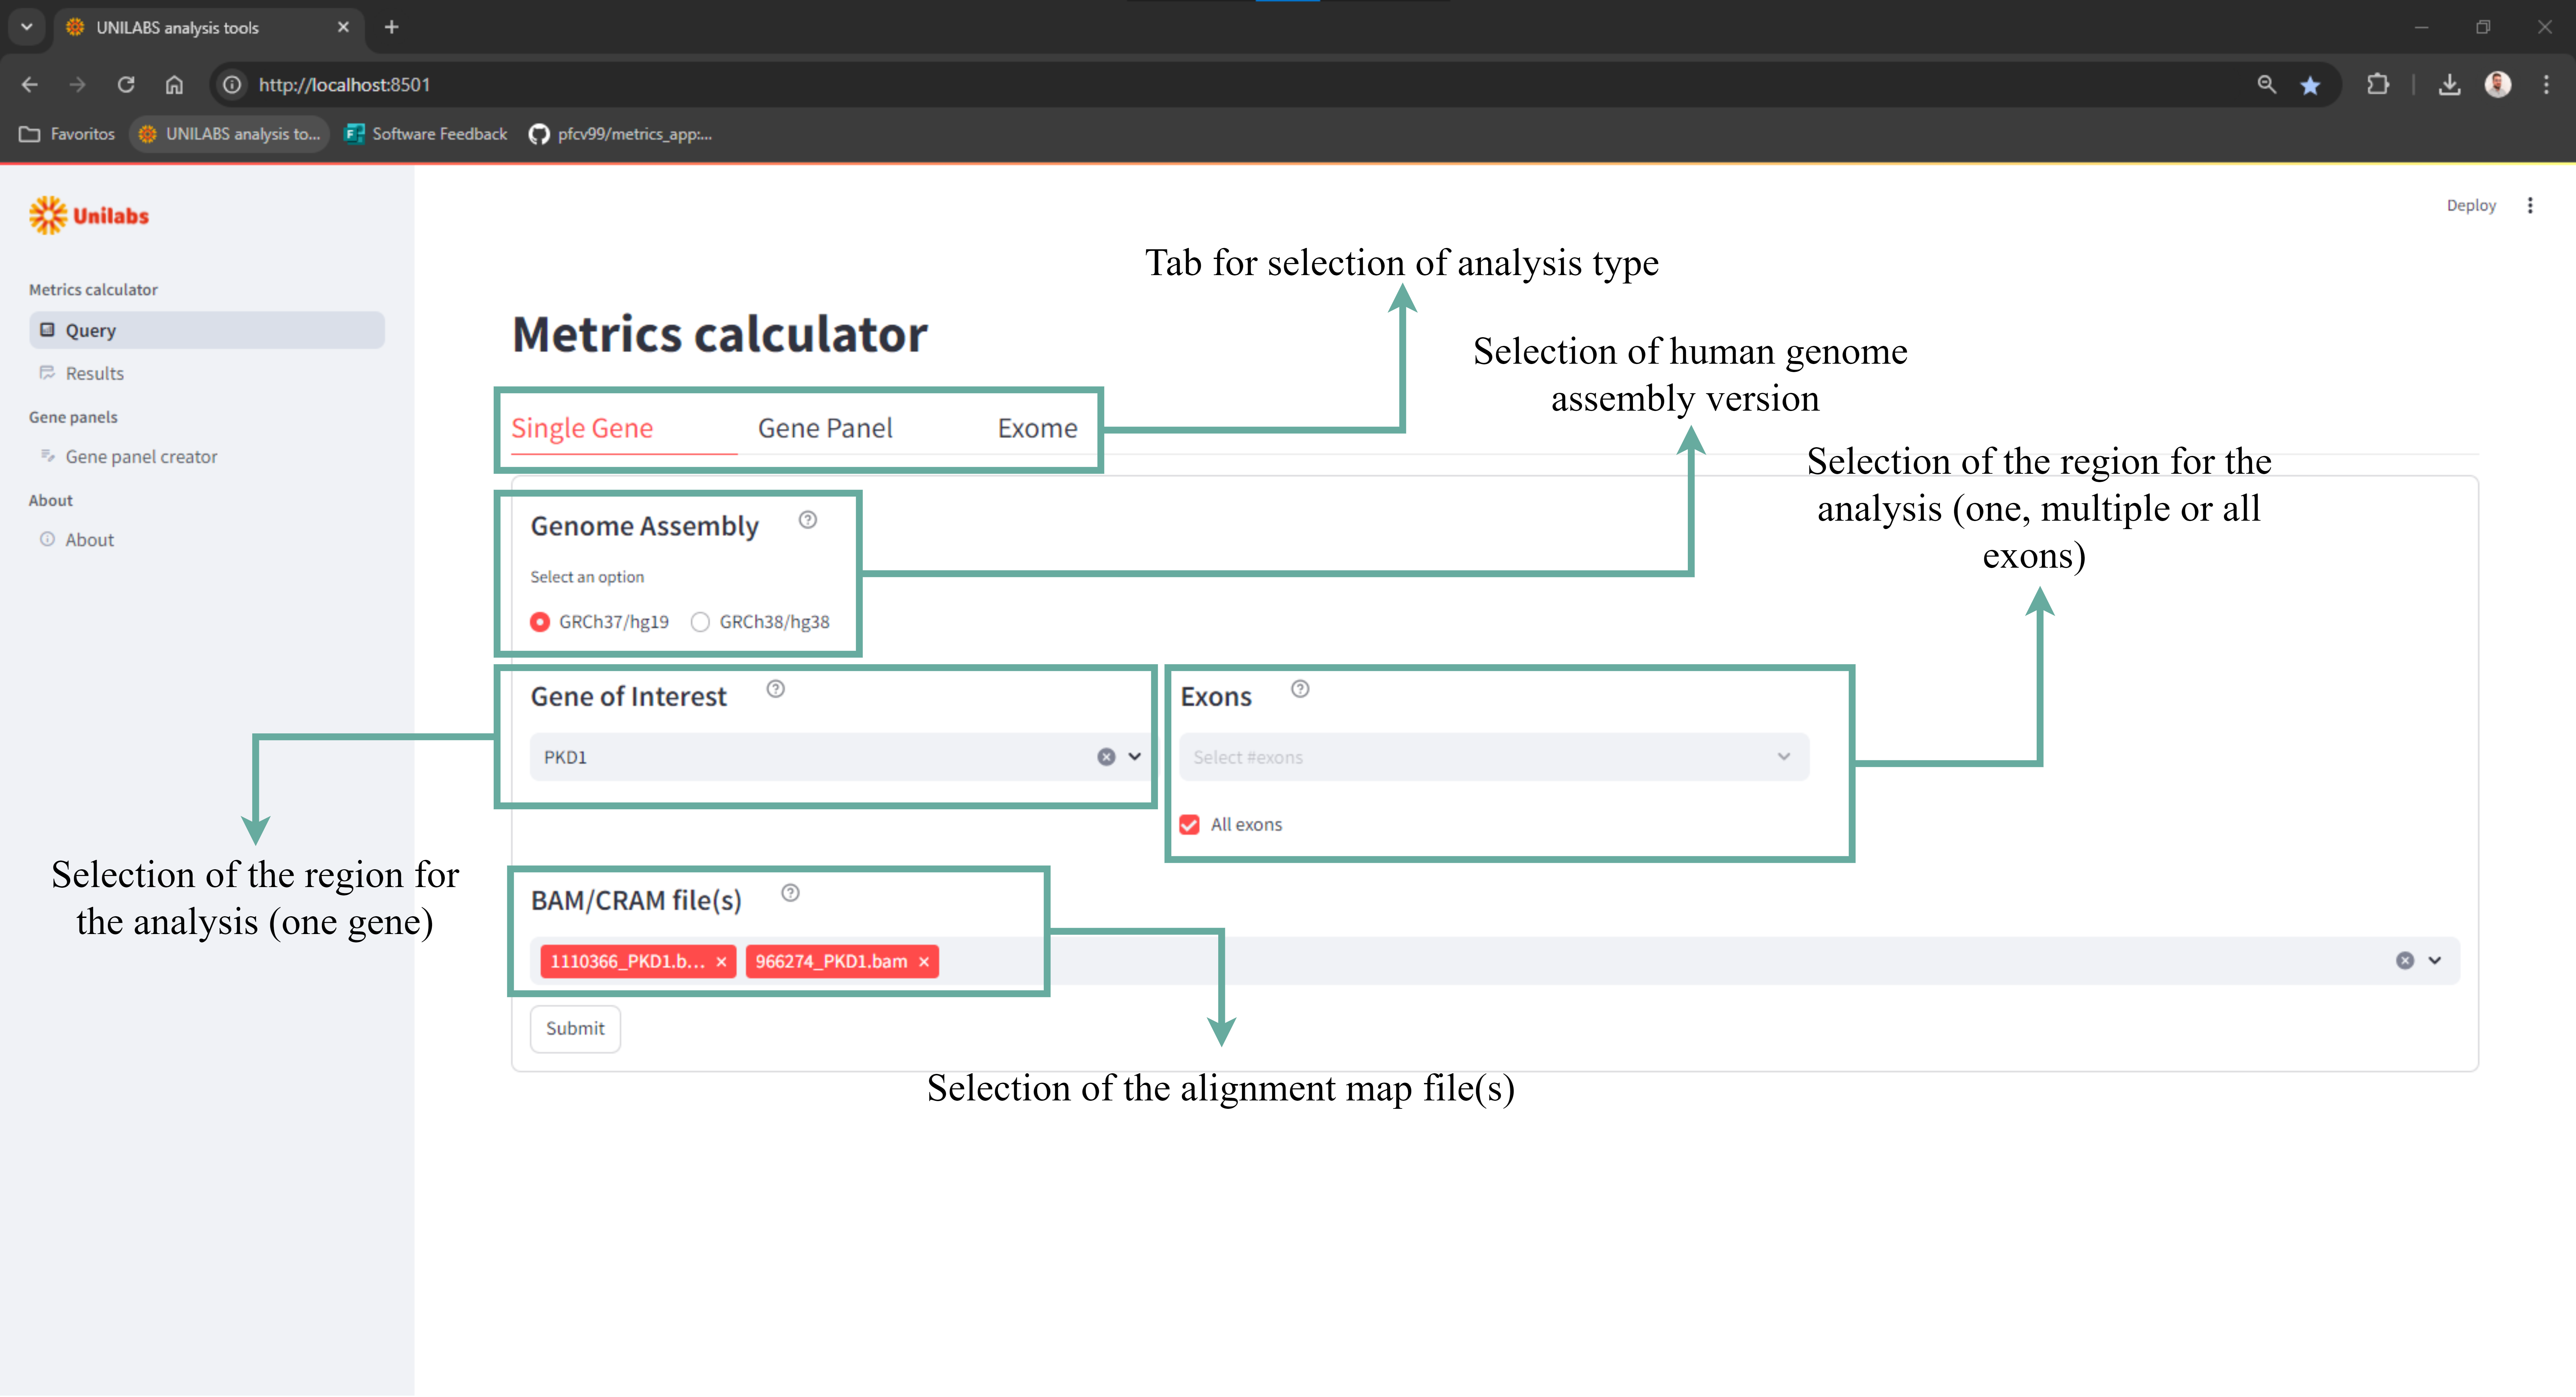
\includegraphics[width=\textwidth]{figs/v3.2.png}
    \caption{Single Gene Analysis Workflow}
    \label{fig:single_gene}
\end{figure}

\begin{itemize}
    \item \textbf{Results and Report Generation}

    Once the data is processed, users can access the results in the \texttt{Results} tab, as seen in Figure \ref{fig:results_loading}. The software compiles a detailed report that includes various metrics such as Average Read Depth, Breadth of Coverage, and Depth of Coverage percentages across different thresholds (e.g., 10x, 20x, 30x). This data is also available for download in a \ac{csv} or \ac{pdf} format, ensuring users can retain a permanent copy of the analysis results.
    
    \begin{figure}[H]
        \centering
        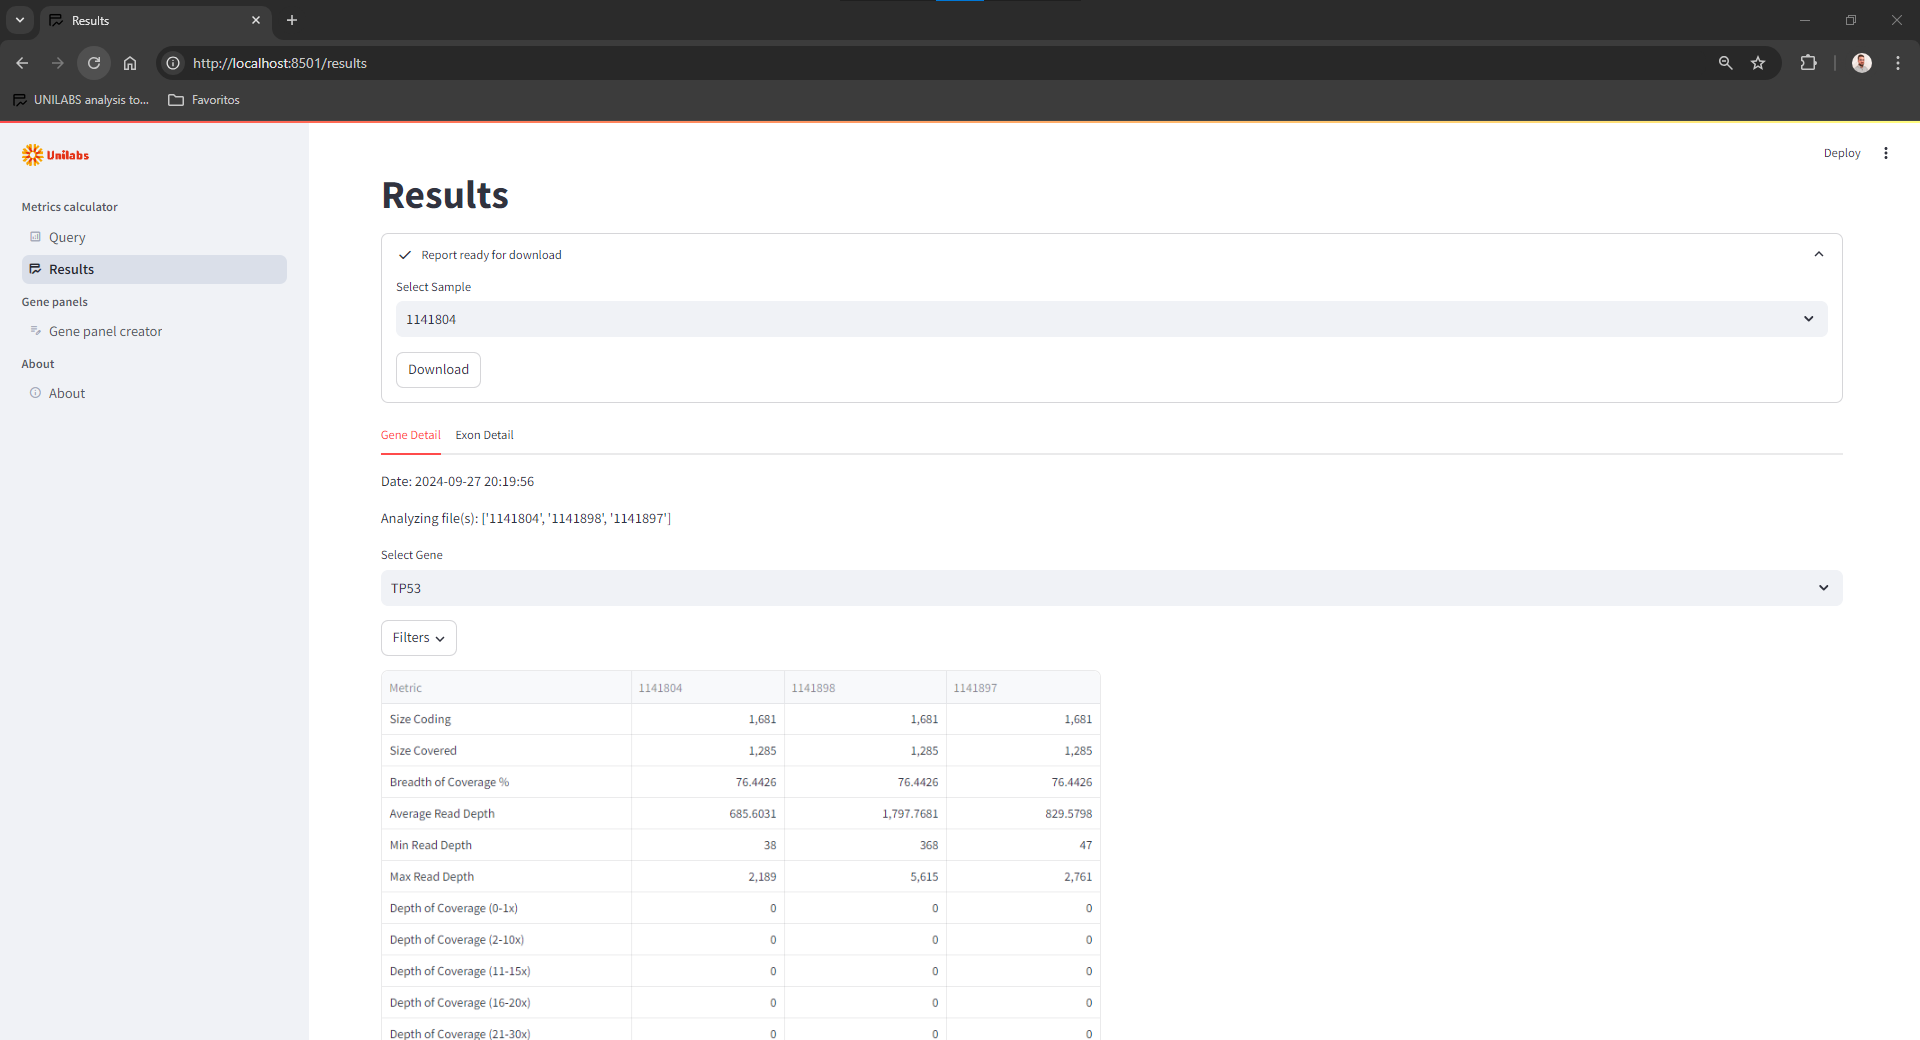
\includegraphics[width=\textwidth]{figs/v3.3.png}
        \caption{Results Tab Loading the Final Report}
        \label{fig:results_loading}
    \end{figure}
    
    In Figure \ref{fig:results_loading} and \ref{fig:final_report}, the detailed metrics for the gene \textit{PKD1} are displayed, offering both gene-level and exon-level statistics. This comprehensive breakdown allows researchers to thoroughly assess the sequencing coverage for the analyzed samples. Key metrics include the Size Coding of the gene, minimum and Maximum Read Depth, and coverage percentages across various depth thresholds, providing valuable insights into the quality and completeness of the sequencing data.
    
    For this case study, the Size Coding of the \textit{PKD1} gene is 14092 \ac{bp}, with a Size Covered of 14092 \ac{bp} for both samples, resulting in a Breadth of Coverage of 100\%. The Average Read Depth across the three samples was 562.58x and 313.98x, respectively. Depth of Coverage, or the number of times a particular region of the genome is covered by reads, directly impacts the reliability of variant detection, gene expression studies, and other genomic analyses. Inconsistent or insufficient depth may lead to variability in the ability to accurately detect mutations or copy number variations, potentially resulting in false positives or false negatives. For instance, lower depth may miss variants that are present at low frequencies, while higher depth ensures that even rare mutations are confidently identified. \cite{Larson2023}
    
    When examining the Depth of Coverage across different thresholds, the percentages for the 10x, 20x, and 30x thresholds were consistently 100\% for both samples, demonstrating that all regions of interest achieved sufficient coverage at these lower thresholds. However, at higher thresholds, the Depth of Coverage showed more variability. For the 50x threshold, the coverage percentages were 99.99\% and 99.47\%, respectively. Similarly, at the 100x threshold, the Depth of Coverage percentages were 98.92\% and 91.69\%. Finally, at the highest threshold of 500x, the coverage percentages dropped more significantly, with values of 51.36\% and 14.66\%, respectively.
    
    \begin{figure}[H]
        \centering
        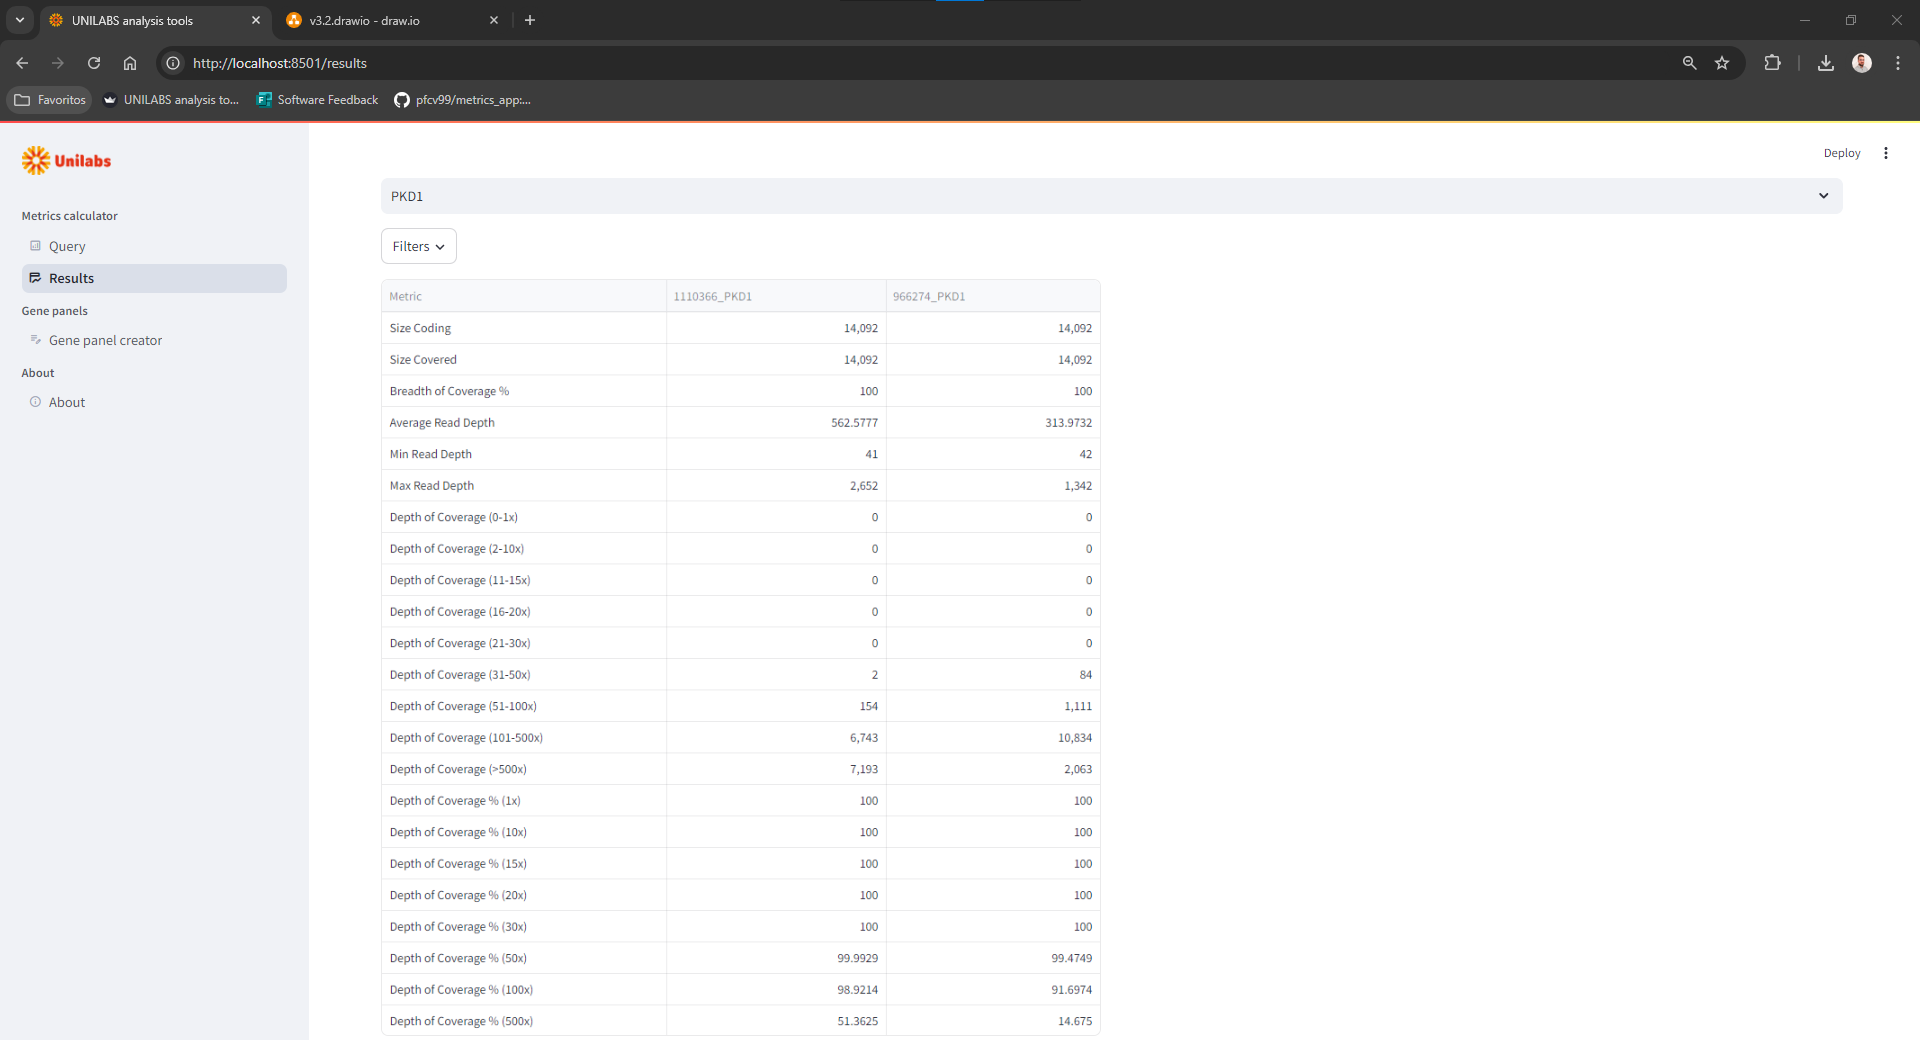
\includegraphics[width=\textwidth]{figs/v3.4.png}
        \caption{Final Report with Detailed Metrics for Gene TP53}
        \label{fig:final_report}
    \end{figure}
    
    \item \textbf{Depth of Coverage Visualization}
    
    One of the critical features of the final software version is its ability to visualize in a plot the distribution of Depth of Coverage across each position, as shown in Figure \ref{fig:coverage_plot}. This visualization allows users to see the depth of sequencing across the gene of interest, with blue regions highlighting exons. A threshold can be set by the user, and regions that fall below this threshold are highlighted in red, ensuring that gaps or low-coverage areas are easily identified. This is particularly important for researchers assessing the completeness of their sequencing data.
    
    \begin{figure}[H]
        \centering
        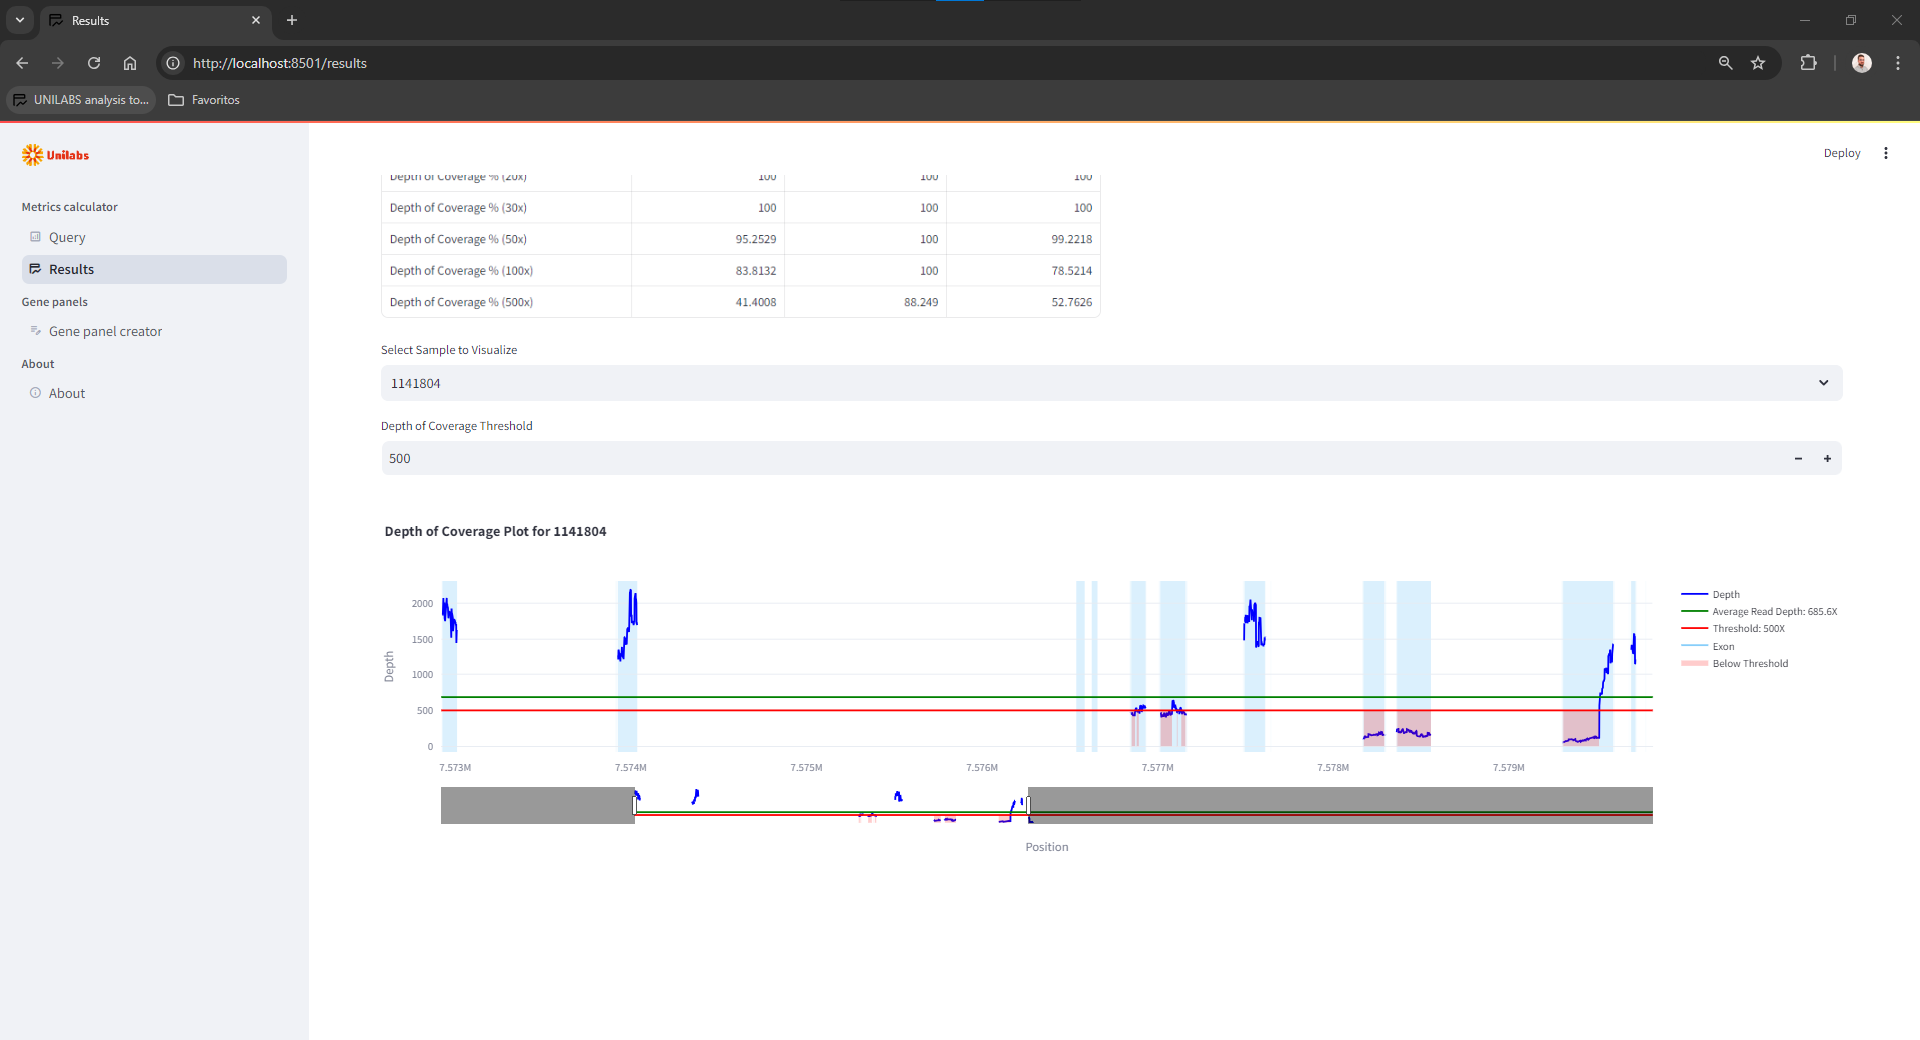
\includegraphics[width=\textwidth]{figs/v3.5.png}
        \caption{Depth of Coverage Visualization for Gene TP53}
        \label{fig:coverage_plot}
    \end{figure}
\end{itemize}

\subsubsection{\textbf{Gene Panel Analysis}}

In the gene panel analysis, the software is configured to process multiple genes simultaneously, as opposed to the single gene analysis. This functionality is particularly useful when studying gene panels associated with specific hereditary diseases, such as the BRCA1 and BRCA2 genes, commonly linked to breast and ovarian cancer. The analysis workflow is similar to that of a single gene but extends to multiple regions of interest, providing broader insights into the Depth and Breadth of Coverage across the entire panel.

\begin{itemize}
\item \textbf{Panel Selection and Input}

The user begins by selecting the appropriate genome assembly and the gene panel of interest. For this case study, the panel for breast and ovarian cancer was selected, which includes 27 genes, among which the BRCA1 and BRCA2 genes. The input consists of a \ac{bam} or \ac{cram} file associated with the selected panel, as shown in Figure \ref{fig:panel_input}.

\begin{figure}[H]
    \centering
    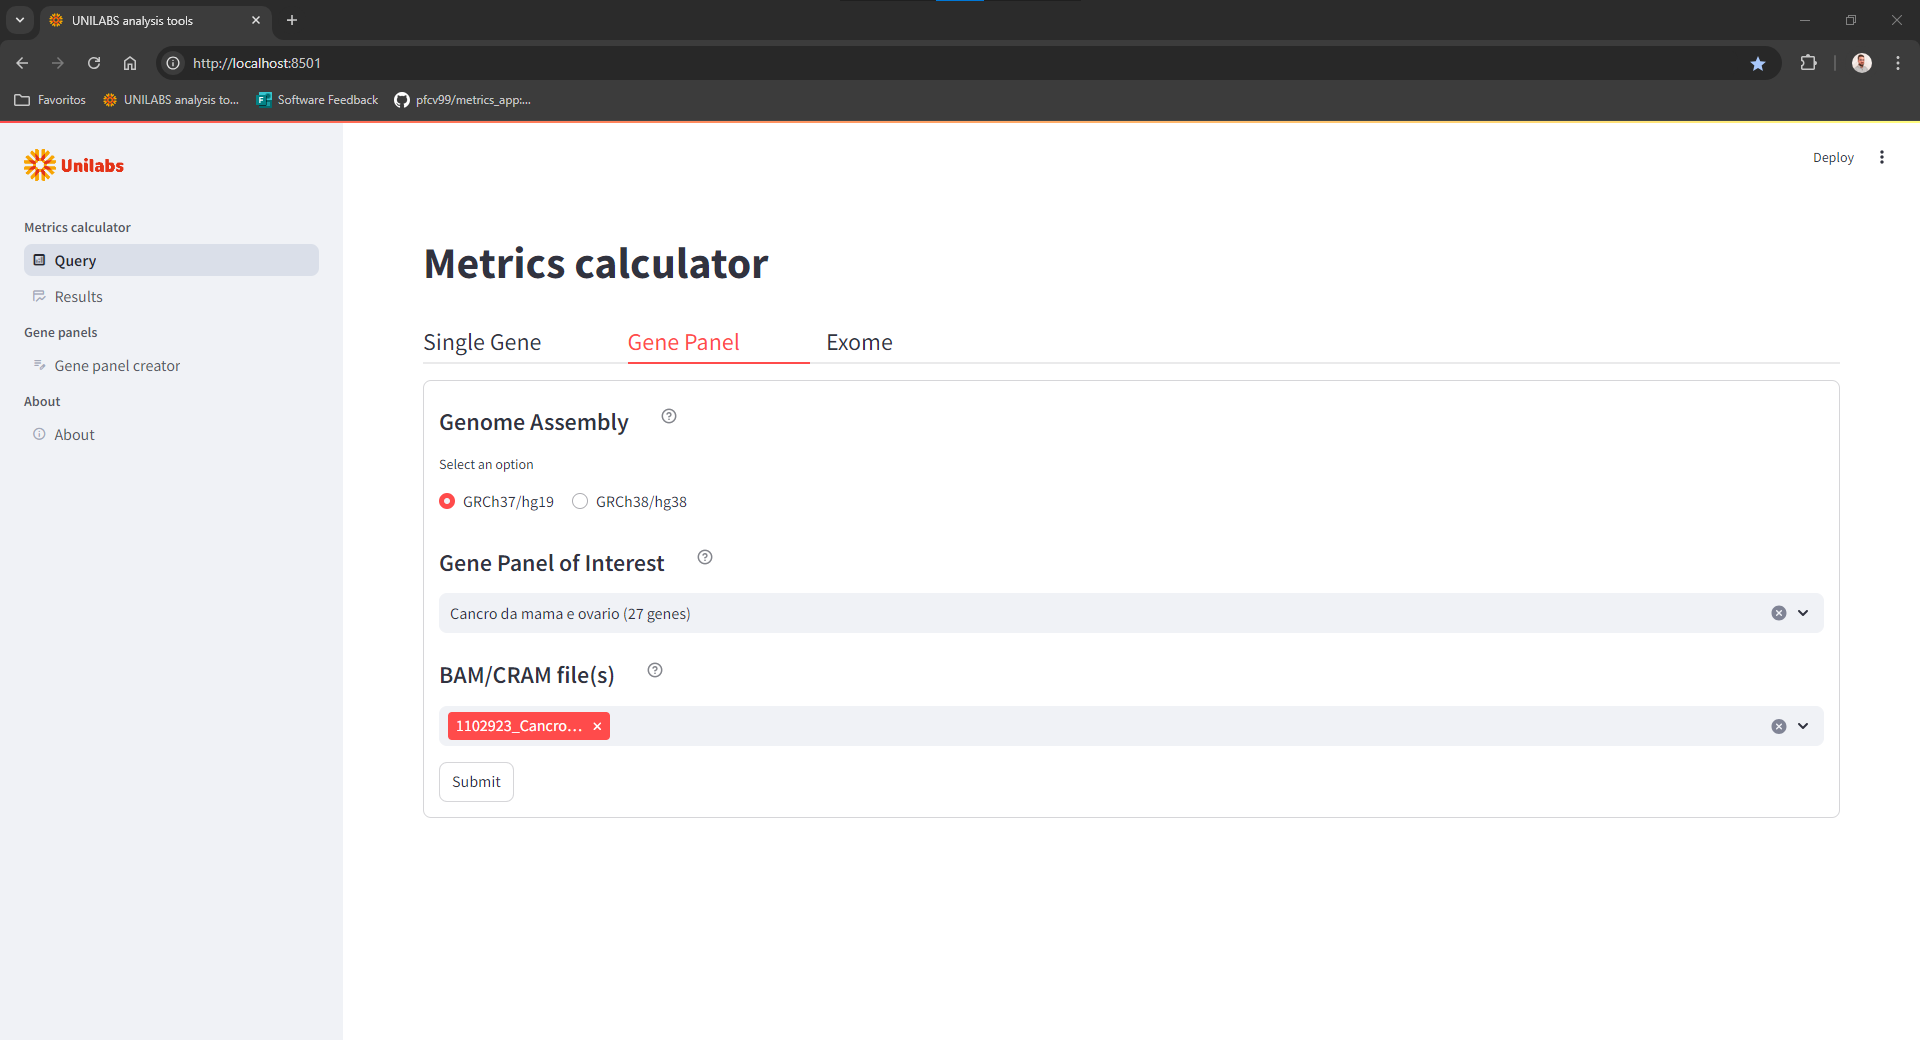
\includegraphics[width=\textwidth]{figs/v3.8.png}
    \caption{Gene Panel Input Selection and Submission}
    \label{fig:panel_input}
\end{figure}

\item \textbf{Overall Results for the Gene Panel}

Once the data is processed, the software generates a comprehensive table of metrics for the entire gene panel. This includes critical metrics such as Size Coding, Size Covered, Breadth of Coverage, and Average Read Depth. These metrics are essential for evaluating the quality of sequencing across all genes in the panel. Figure \ref{fig:panel_results_overall} illustrates the results generated for the gene panel associated with hereditary breast and ovarian cancer. For this specific case, a panel with a Size Coding of 119175 \ac{bp}, the Size Covered was 93043 \ac{bp}, resulting in a Breadth of Coverage of 78.07\%. The Average Read Depth across the panel was 263.93x, with a Minimum Read Depth of 1x and a Maximum Read Depth of 631x. The Depth of Coverage across different thresholds revealed that the panel achieved a Depth of Coverage between 87.28\% and 100\% at the 1x, 10x and 15x, 20x, 30x, 50x and 100x threshold. For the 500x threshold, the Depth of Coverage percentage dropped to 1.9\%, indicating regions less covered by sequencing. 

\begin{figure}[H]
    \centering
    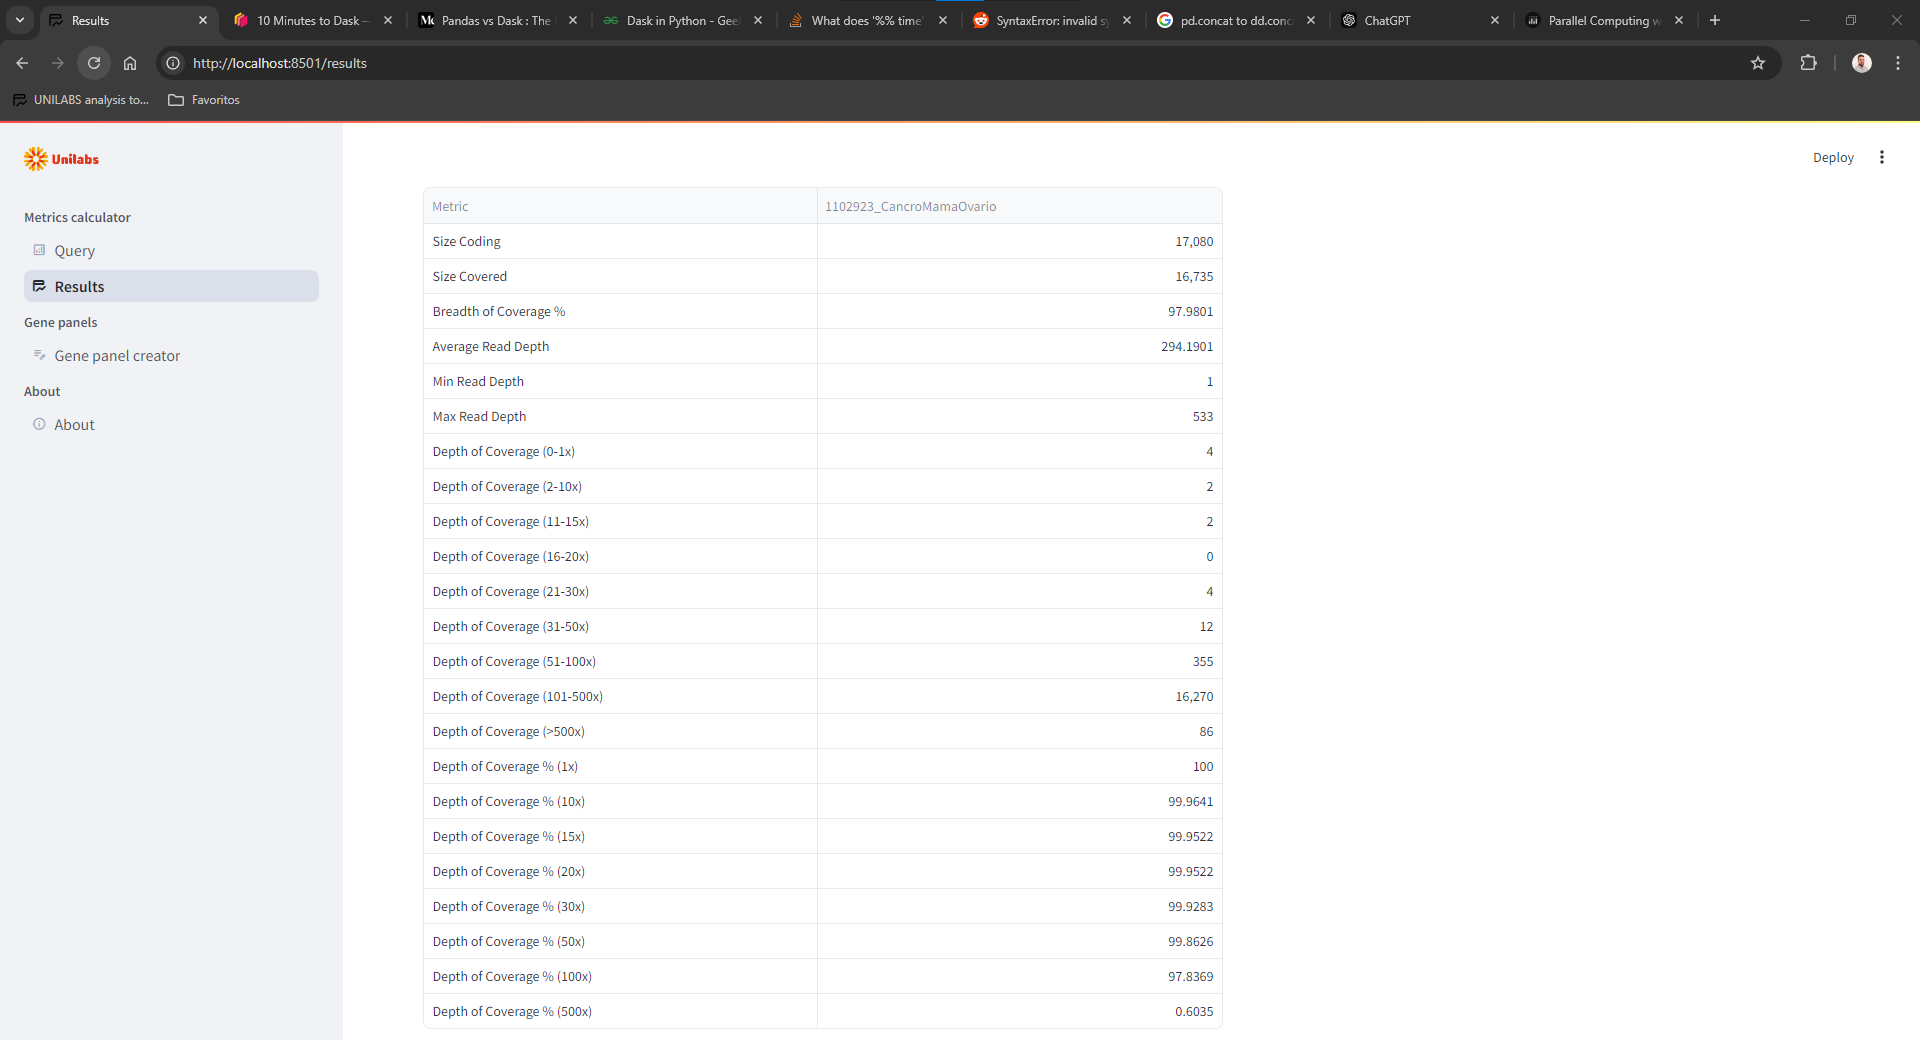
\includegraphics[width=\textwidth]{figs/v3.9.png}
    \caption{Overall Gene Panel Results for Hereditary Breast and Ovarian Cancer}
    \label{fig:panel_results_overall}
\end{figure}

\item \textbf{Individual Gene Metrics}

The software allows users to dive deeper into the metrics for individual genes within the panel. Figure \ref{fig:brca1_results} displays the results for the BRCA1 gene. The Size Coding of BRCA1 was 6343 \ac{bp}, with a Size Covered of 6124 \ac{bp}, resulting in a Breadth of Coverage of 96.5\%. The Average Read Depth for BRCA1 was 345.3x, with a Minimum Read Depth of 1x and a Maximum Read Depth of 533x. The Depth of Coverage across different thresholds showed consistent percentages above 99\% for the 1x, 10x,, 15x, 20x, 30x, 50x and 100x thresholds, with a slight drop to 1.6\% at the 500x threshold.

\begin{figure}[H]
    \centering
    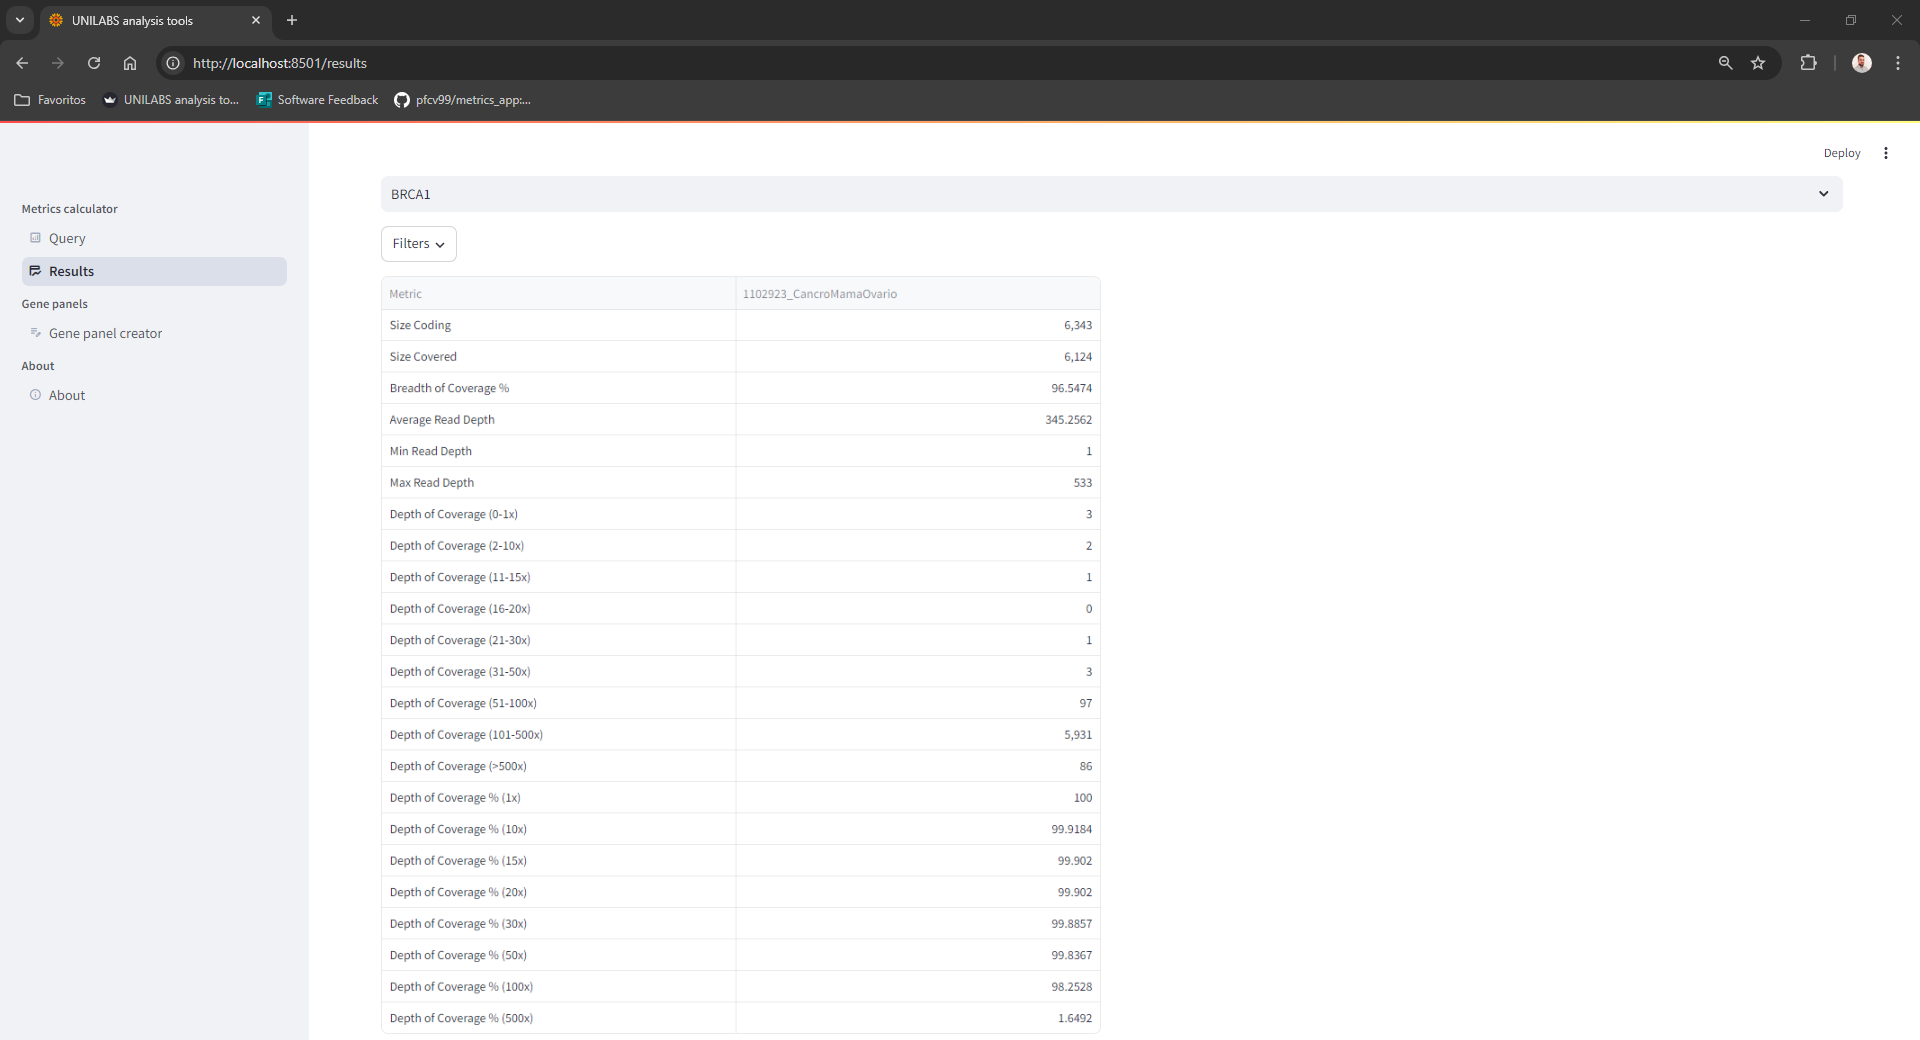
\includegraphics[width=\textwidth]{figs/v3.10.png}
    \caption{Detailed Metrics for the BRCA1 Gene}
    \label{fig:brca1_results}
\end{figure}

\item \textbf{Exon-Level Analysis}

In addition to gene-level metrics, the software also offers exon-level analysis. Users can select specific exons within the genes to obtain a more granular view of the sequencing Depth of Coverage. This level of detail is particularly useful when assessing the completeness of the sequencing across critical regions within each gene. Figure \ref{fig:exon_results} shows the results for the 13rd exon of the BRCA1 gene, where key metrics are also displayed. This exon-level detail allows researchers to pinpoint regions that may require additional sequencing or validation. For the 13rd exon of BRCA1, the Size Coding was 126 \ac{bp}, with a Size Covered of 126 \ac{bp}, resulting in a Breadth of Coverage of 100\%. The Average Read Depth for this exon was 261.98x, with a Minimum Read Depth of 216x and a Maximum Read Depth of 291x. The Depth of Coverage across different thresholds showed consistent coverage percentages of 100\% for the 1x, 10x, 15x, 20x, 30x, 50x, 100x thresholds, with a drop to 0\% at the 500x threshold.

\begin{figure}[H]
    \centering
    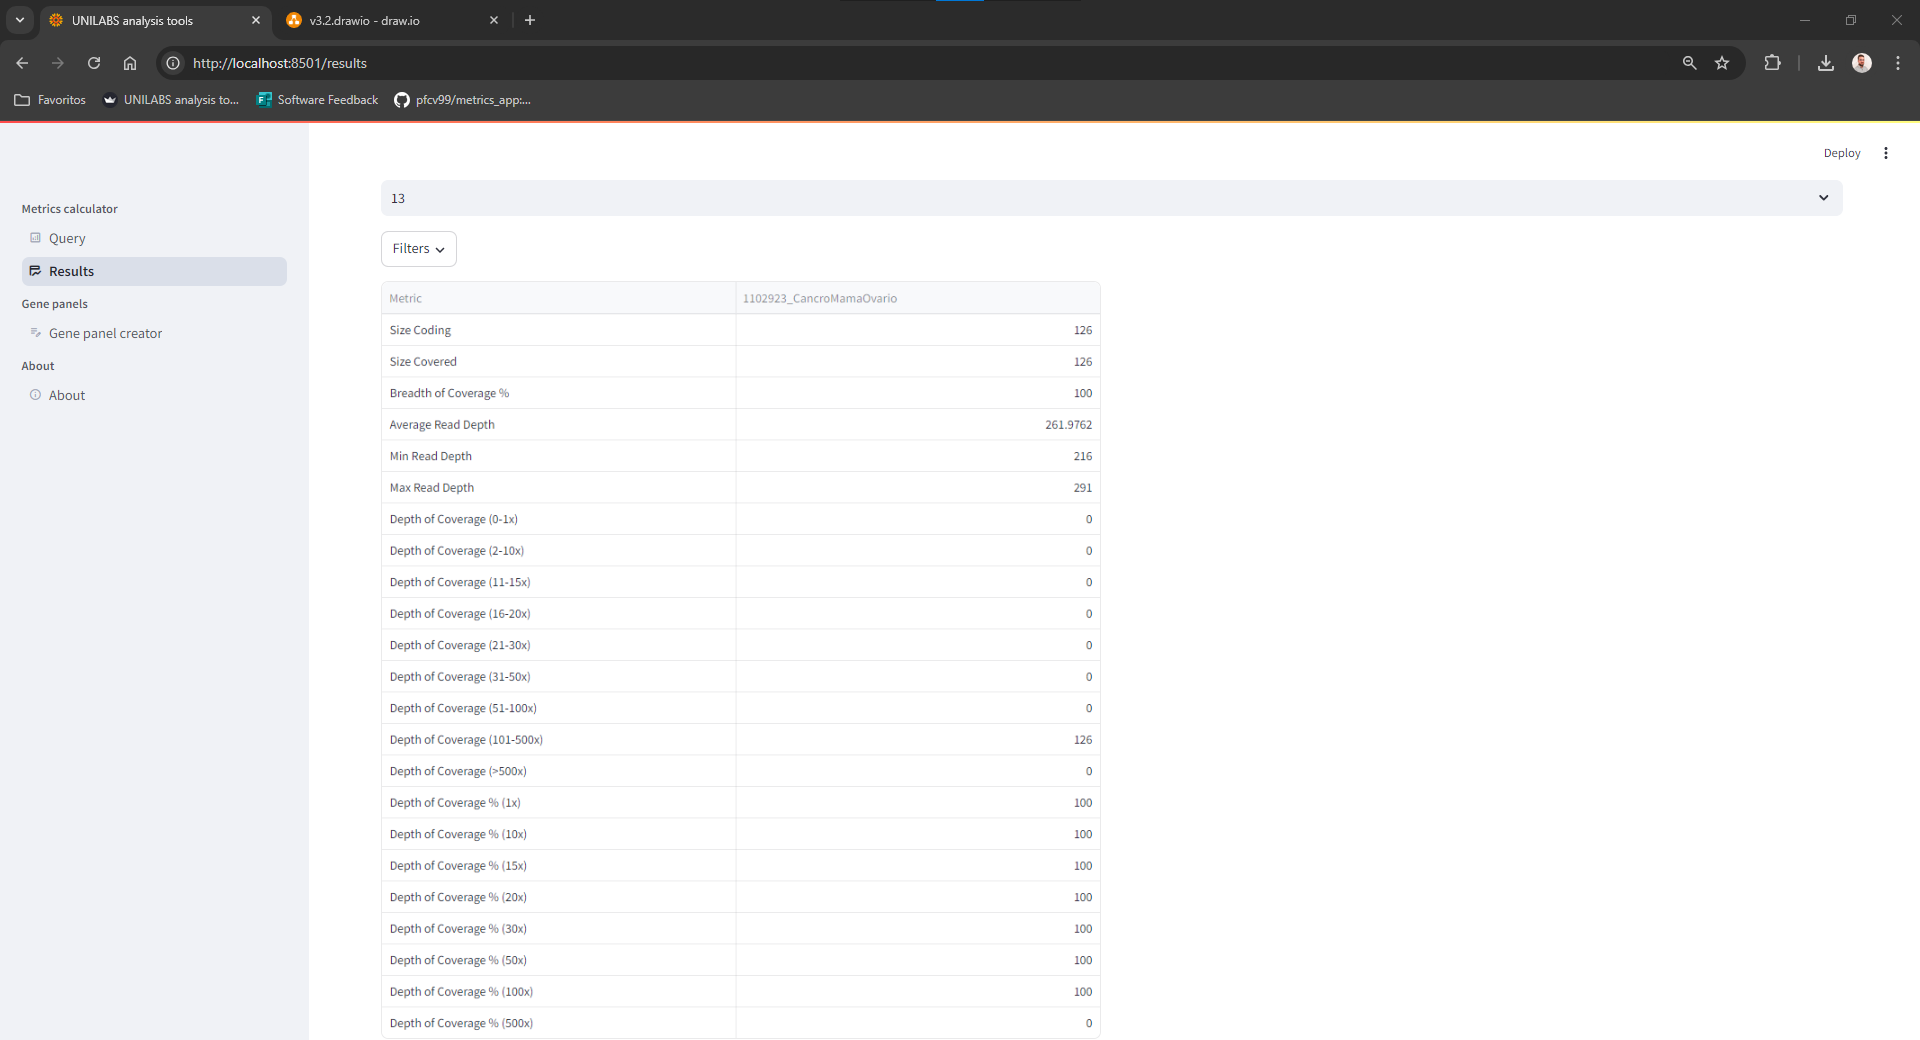
\includegraphics[width=\textwidth]{figs/v3.12.png}
    \caption{Exon-Level Metrics for the BRCA1 Gene}
    \label{fig:exon_results}
\end{figure}

The gene panel analysis feature provides a powerful tool for evaluating sequencing coverage across multiple genes simultaneously. By offering both gene-level and exon-level insights, the software ensures that researchers can thoroughly assess the quality of their sequencing data, identify potential gaps in coverage, and make informed decisions regarding further analysis or re-sequencing.

\end{itemize}

\section{Test and Validation}

To validate the tool, each \ac{bam} file was analyzed using the commercial software Omnomics, and the results were compared with those obtained from the developed software. The analyses were performed separately for a Single Gene and a Gene Panel, ensuring that each \ac{bam} file was used for its respective analysis.

\subsection{Single Gene Analysis}

The gene TP53 was selected for the Single Gene analysis, and the results obtained from the developed software were compared with those from Omnomics. The metrics compared included Average Read Depth and Depth of Coverage \% (1x, 10x, 20x, 30x, 50x, 100x, 500x).

\begin{table}[H]
    \centering
    \caption{Comparison of Metrics between the developed software and Omnomics for Gene TP53}
    \label{tab:omnomicsVSunilabs}
    \begin{tabular}{@{}lrr@{}}
    \toprule
    \textbf{Metric}             & \textbf{Developed software} & \textbf{Omnomics} \\ \midrule
    Average Read Depth          & 874,97                      & 891               \\
    Depth of Coverage \% (1x)   & 99.86                       & 100               \\
    Depth of Coverage \% (10x)  & 99.86                       & 100               \\
    Depth of Coverage \% (20x)  & 99.86                       & 100               \\
    Depth of Coverage \% (30x)  & 99.86                       & 100               \\
    Depth of Coverage \% (50x)  & 99.86                       & 100               \\
    Depth of Coverage \% (100x) & 99.79                       & 99.90             \\
    Depth of Coverage \% (500x) & 57.42                       & 59                \\ \bottomrule
    \end{tabular}
    \end{table}

The comparison of results between the two software solutions reveals some minor discrepancies. In the Average Read Depth metric, the developed software reported an average depth of 874.97, whereas Omnomics recorded a slightly higher value of 891. These differences can be primarily attributed to the variations in the reference \ac{bed} files used by each tool. The developed software relies on an optimized \ac{bed} file from \ac{mane}, while Omnomics utilizes a GENCODE \ac{bed} created through the Table Browser tool of the Genome Browser, specifically targeting the TP53 gene with an extension of 8 base pairs. These differing \ac{bed} files lead to variations in the covered regions, directly influencing metrics such as Average Read Depth.

Both tools exhibited identical results for the Depth of Coverage percentages across lower thresholds, including 1x, 10x, 20x, 30x, and 50x, demonstrating full coverage at these depths. However, slight deviations are noted at higher coverage thresholds. For instance, the Depth of Coverage percentage at 100x reveals minimal differences, with the developed software reporting 99.79\% and Omnomics reporting 99.9\%.

A more noticeable difference is observed in the Depth of Coverage percentage at 500x, where the developed software reported 57.42\%, compared to Omnomics 59\%. This discrepancy can once again be attributed to the differing regions encompassed by the respective \ac{bed} files, which affect the depth distribution across the analyzed regions.

Overall, by comparing the developed tool with Omnomics, it was possible to infere that the developed software is capable of providing accurate and reliable metrics for Single Gene analysis. The variations observed in the results are primarily due to differences in the reference \ac{bed} files used by each tool, highlighting the importance of selecting the appropriate reference file for accurate coverage analysis.

\subsection{Gene Panel Analysis}

For the analysis of a gene panel the previous panel "Cancro da mama e ovário (27 genes)" was used. One of the \ac{bam} files used was compared between the the developed software and the commercial tool Omnomics. The results are detailed in Table \ref{tab:panel_omnomicsVSunilabs}, highlighting the differences between the two tools for several metrics.

\begin{table}[H]
    \centering
    \caption{Comparison of Metrics between the developed software and Omnomics for Gene Panel: Cancro da mama e ovário (27 genes)}
    \label{tab:panel_omnomicsVSunilabs}
    \begin{tabular}{@{}lrr@{}}
    \toprule
    \textbf{Metric}             & \textbf{Developed software} & \textbf{Omnomics} \\ \midrule
    Average Read Depth          & 263.93                      & 388               \\
    Depth of Coverage \% (1x)   & 100                         & 99.60             \\
    Depth of Coverage \% (10x)  & 95.19                       & 99.50             \\
    Depth of Coverage \% (20x)  & 93.69                       & 99.40             \\
    Depth of Coverage \% (30x)  & 92.78                       & 99.20             \\
    Depth of Coverage \% (50x)  & 91.21                       & 98.80             \\
    Depth of Coverage \% (100x) & 87.28                       & 96.10             \\
    Depth of Coverage \% (500x) & 1.89                        & 27.60             \\ \bottomrule
    \end{tabular}
    \end{table}
    
    The comparison between the developed software and Omnomics for this gene panel reveals several key differences in the reported metrics. Most notably, the Average Read Depth shows a significant disparity, with the developed software reporting a depth of 263.93, while Omnomics reports a substantially higher value of 388. This difference can once again be attributed to the different \ac{bed} files used by each tool.
    
    For the Depth of Coverage \% metrics, both tools report similar values, though some minor differences are present. At the 1x coverage threshold, the developed software reports 100\%, while Omnomics reports 99.6\%. Similarly, for the 10x, 20x, 30x, and 50x thresholds, the differences remain small, with Omnomics consistently reporting slightly higher percentages. However, at the 100x threshold, the tools report nearly identical values, with the developed software at 87.28\% and Omnomics at 96.1\%.
    
    The most significant divergence occurs at the 500x threshold. The developed software reports a very low value of 1.89\%, while Omnomics reports a much higher 27.6\%. This discrepancy is likely due to the differing regions targeted by the \ac{bed} files, with Omnomics potentially including regions of higher coverage within the panel that are not present in the MANE \ac{bed} file used by the developed software.
    
    Overall, the comparison between the two tools highlights, once again, the importance of the reference \ac{bed} file used in determining coverage metrics. While the results are largely consistent across most coverage thresholds, notable differences, particularly in the Average Read Depth and the highest coverage levels, underscore the impact of \ac{bed} file selection on the analysis results.
    

\section{Performance}

This section presents the performance analysis of the software for both single gene and gene panel analyses. The tests were carried out manually using different sample sizes to evaluate the scalability of the software and the impact on execution time, \ac{cpu} usage, and memory consumption. Two scenarios were tested: the "Single Gene" analysis for the JAK2 gene with 1, 10, and 20 samples, and the "Gene Panel" analysis for the "Breast Cancer Panel," which includes 27 genes, with 1 and 2 samples.

\subsection{Single Gene Analysis: JAK2}

The results for the single gene analysis are summarized in Table \ref{tab:single-gene-performance}. The execution time, \ac{cpu} usage, and memory usage were measured for three main functions: loading the Streamlit interface, running the \texttt{samtools depth} function, and generating the final report and coverage plots. As the number of samples increased, a clear growth in resource usage was observed.

For the "Streamlit load" function, the execution time remained relatively consistent across the different sample sizes, ranging from 0.28 to 0.29 seconds, with \ac{cpu} usage stabilizing around 11-12\%. Memory usage remained between 12.51 \ac{mb} and 12.95 \ac{mb}, showing minor variation as the number of samples increased.

The \texttt{samtools depth} function exhibited significant variability depending on the number of samples. With only 1 sample, the execution time was 0.32 seconds, but it increased substantially to 5.41 seconds with 20 samples. Similarly, \ac{cpu} usage rose from 0.90\% to 1.80\%, and memory usage increased from 4.46 \ac{mb} to 11.15 \ac{mb}, highlighting the resource intensiveness of this operation as more samples were processed.

The report generation phase also experienced an increase in resource demand. The execution time grew from 1.47 seconds for a single sample to 1.85 seconds for 20 samples, while \ac{cpu} usage and memory usage saw corresponding rises, particularly memory consumption, which peaked at 19.30 \ac{mb} for 20 samples.

\begin{table}[htbp] 
    \centering 
    \caption{Performance of Single Gene Analysis (JAK2) for 1, 10, and 20 Samples}
    \label{tab:single-gene-performance}
    \resizebox{\textwidth}{!}{%
    \begin{tabular}{@{}l>{\raggedleft\arraybackslash}p{1cm}>{\raggedleft\arraybackslash}p{1cm}>{\raggedleft\arraybackslash}p{1cm}>{\raggedleft\arraybackslash}p{1cm}>{\raggedleft\arraybackslash}p{1cm}>{\raggedleft\arraybackslash}p{1cm}>{\raggedleft\arraybackslash}p{1cm}>{\raggedleft\arraybackslash}p{1cm}>{\raggedleft\arraybackslash}p{1cm}@{}}
    \toprule
    \textbf{Function} & \multicolumn{3}{c}{\textbf{Execution Time (s)}} & \multicolumn{3}{c}{\textbf{\ac{cpu} usage (\%)}} & \multicolumn{3}{c}{\textbf{Memory Usage (\ac{mb})}} \\ \midrule
    Streamlit load            & 0.28 & 0.28 & 0.29  & 11.20 & 11.90 & 12.30 & 12.51 & 12.58 & 12.95  \\
    Samtools depth function    & 0.32 & 3.26 & 5.41  & 0.90  & 1.70  & 1.80  & 4.46  & 7.58  & 11.15  \\
    Report build               & 1.47 & 1.67 & 1.85  & 2.10  & 3.00  & 4.00  & 7.96  & 10.33 & 19.30  \\ 
    Coverage plot generation   & 0.33 & -    & -     & 4.20  & -     & -     & 1.93  & -     & -      \\ \midrule
    \textbf{No of samples}     & 1    & 10   & 20    & 1     & 10    & 20    & 1     & 10    & 20     \\ \bottomrule
    \end{tabular}
    }
\end{table}

\subsection{Gene Panel Analysis: Breast Cancer Panel}

Table \ref{tab:gene-panel-performance} presents the performance results for the "Breast Cancer Panel" analysis, which contains 27 genes, for 1 and 2 samples. As expected, increasing the number of samples caused a noticeable rise in execution time, \ac{cpu} usage, and memory consumption across all measured functions.

For the "Streamlit load" function, the execution time remained almost constant, ranging from 0.27 seconds for 1 sample to 0.30 seconds for 2 samples. \ac{cpu} and memory usage followed a similar pattern, showing little variation between the two sample sizes.

The \texttt{samtools depth} function exhibited a significant increase in both execution time and resource usage when moving from 1 to 2 samples. The execution time grew from 4.36 seconds to 11.47 seconds, while \ac{cpu} usage increased from 1.80\% to 3.30\%. Memory usage also rose, from 5.93 \ac{mb} for 1 sample to 6.33 \ac{mb} for 2 samples.

The report generation function showed a substantial increase in both execution time and resource usage, with the execution time rising from 9.88 seconds for 1 sample to 24.46 seconds for 2 samples. \ac{cpu} usage increased from 6.50\% to 8.30\%, and memory consumption surged from 1.52 \ac{mb} to 29.19 \ac{mb}, indicating that this function is particularly resource-intensive with larger datasets.

\begin{table}[htbp] 
    \centering 
    \caption{Performance of Gene Panel Analysis (Breast Cancer Panel) for 1 and 2 Samples}
    \label{tab:gene-panel-performance}
    \resizebox{\textwidth}{!}{%
    \begin{tabular}{@{}l>{\raggedleft\arraybackslash}p{1cm}>{\raggedleft\arraybackslash}p{1cm}>{\raggedleft\arraybackslash}p{1cm}>{\raggedleft\arraybackslash}p{1cm}>{\raggedleft\arraybackslash}p{1cm}>{\raggedleft\arraybackslash}p{1cm}@{}}
    \toprule
    \textbf{Function} & \multicolumn{2}{c}{\textbf{Execution Time (s)}} & \multicolumn{2}{c}{\textbf{\ac{cpu} usage (\%)}} & \multicolumn{2}{c}{\textbf{Memory Usage (\ac{mb})}} \\ \midrule
    Streamlit load           & 0.27 & 0.30  & 11.25 & 10.90 & 12.21 & 12.02 \\
    Samtools depth function  & 4.36 & 11.47 & 1.80  & 3.30  & 5.93  & 6.33  \\
    Report build             & 9.88 & 24.46 & 6.50  & 8.30  & 1.52  & 29.19 \\ \midrule
    \textbf{No of samples}   & 1    & 2     & 1     & 2     & 1     & 2     \\ \bottomrule
    \end{tabular}% 
    }
\end{table}

The performance analysis of the software shows that it scales predictably with the number of samples processed, particularly in the \texttt{samtools depth} and report generation functions. The "Single Gene" analysis, while resource-efficient for a small number of samples, exhibits a noticeable increase in execution time and resource consumption as the sample size grows, particularly in the depth calculation function. 

For the "Gene Panel" analysis, which involves a more complex dataset (27 genes), the resource usage for even a small number of samples is significantly higher than for single gene analyses. The report generation function, in particular, exhibits substantial growth in both \ac{cpu} and memory usage, which may indicate a need for optimization in future versions of the software to handle larger datasets more efficiently.


\section{Users feedback}

In order to evaluate the usability and effectiveness of the developed software, a feedback questionnaire was designed and distributed to a group of 14 users from Unilabs Genetics team with diverse professional backgrounds. The primary objective of this questionnaire was to gather insights into the user experience, performance, and overall satisfaction with the software. Given that the software was intended to cater to a wide range of technical expertise, from laboratory technicians to bioinformatics specialists, it was crucial to ensure that it met the functional and usability needs of these varied audiences.

The questionnaire consisted of multiple sections aimed at assessing specific aspects of the software, including the ease of navigation, clarity of the interface, speed of performance, and the usefulness of the analytical metrics provided. Participants were asked to rate their experience on a numerical scale while also providing qualitative feedback on areas where the software excelled or required improvement. The results from these ratings are visually represented in the following figures:

\begin{figure}[H] 
    \centering 
    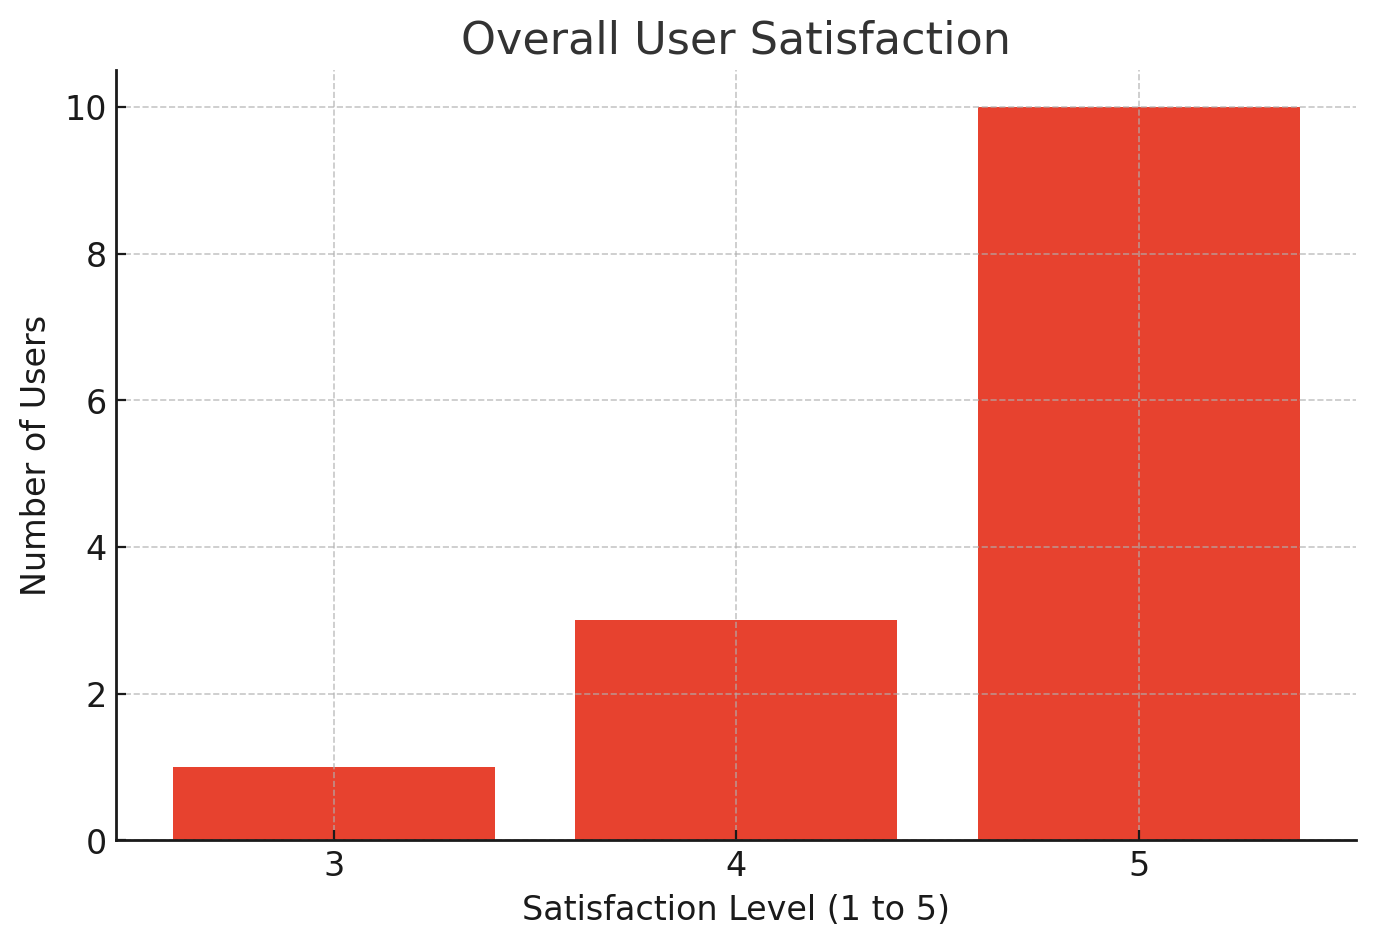
\includegraphics[width=0.6\textwidth]{figs/overall_satisfaction_graph.png} 
    \caption{Overall User Satisfaction Ratings.} 
    \label{fig:overall_satisfaction}
\end{figure}

Figure \ref{fig:overall_satisfaction} shows the distribution of user satisfaction ratings, where most users rated their experience between 4 and 5, indicating a high level of overall satisfaction.

In addition to rating the software's technical performance, respondents were encouraged to share their thoughts on the software's design, user interface, and the clarity of instructions provided throughout the analysis process. This approach allowed for a comprehensive evaluation that encompassed both the functional and aesthetic dimensions of the user experience. The ultimate goal of this survey was to identify key areas that could be optimized to further align the software with the needs of its users, while also validating its current performance and utility in the field of genomic analysis.

In terms of performance, the software was well-regarded for its speed and efficiency, as depicted in Figure \ref{fig:performance}:

\begin{figure}[H] 
    \centering 
    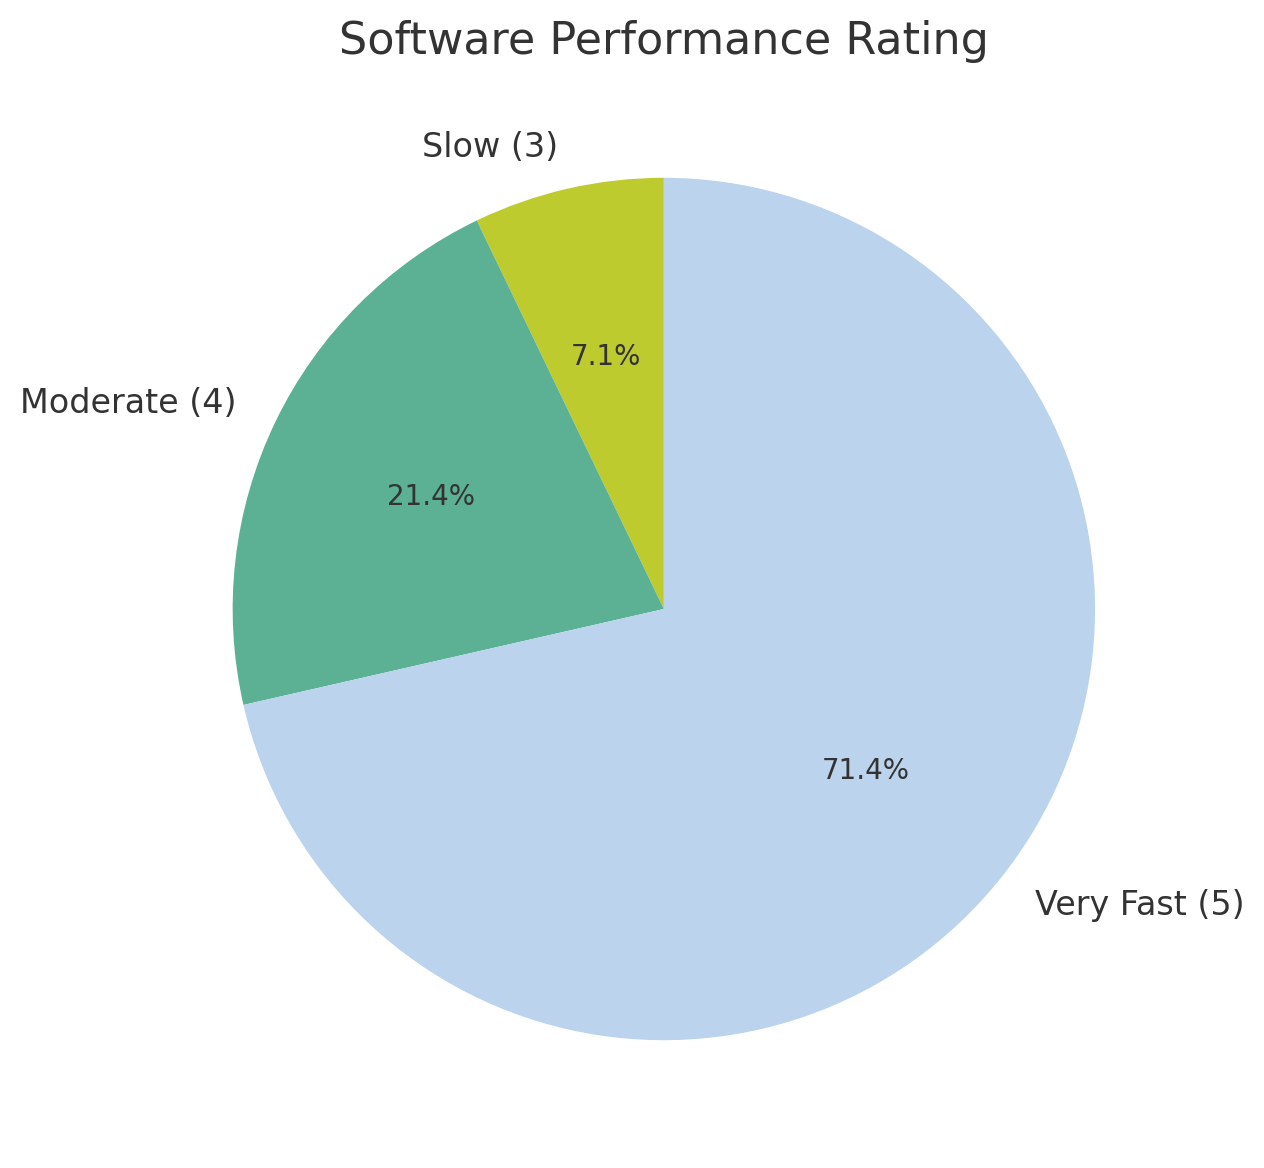
\includegraphics[width=0.6\textwidth]{figs/performance_pie_chart.png} 
    \caption{Performance Ratings for the Software.}
    \label{fig:performance}
\end{figure}

The majority of users rated the software's performance positively, with most respondents giving it a "Fast" or "Very Fast" rating. The clear separation of user ratings shows that speed was a strong positive aspect of the software.

The analysis of the usability of the software is represented in Figure \ref{fig:usability}:

\begin{figure}[H] 
    \centering 
    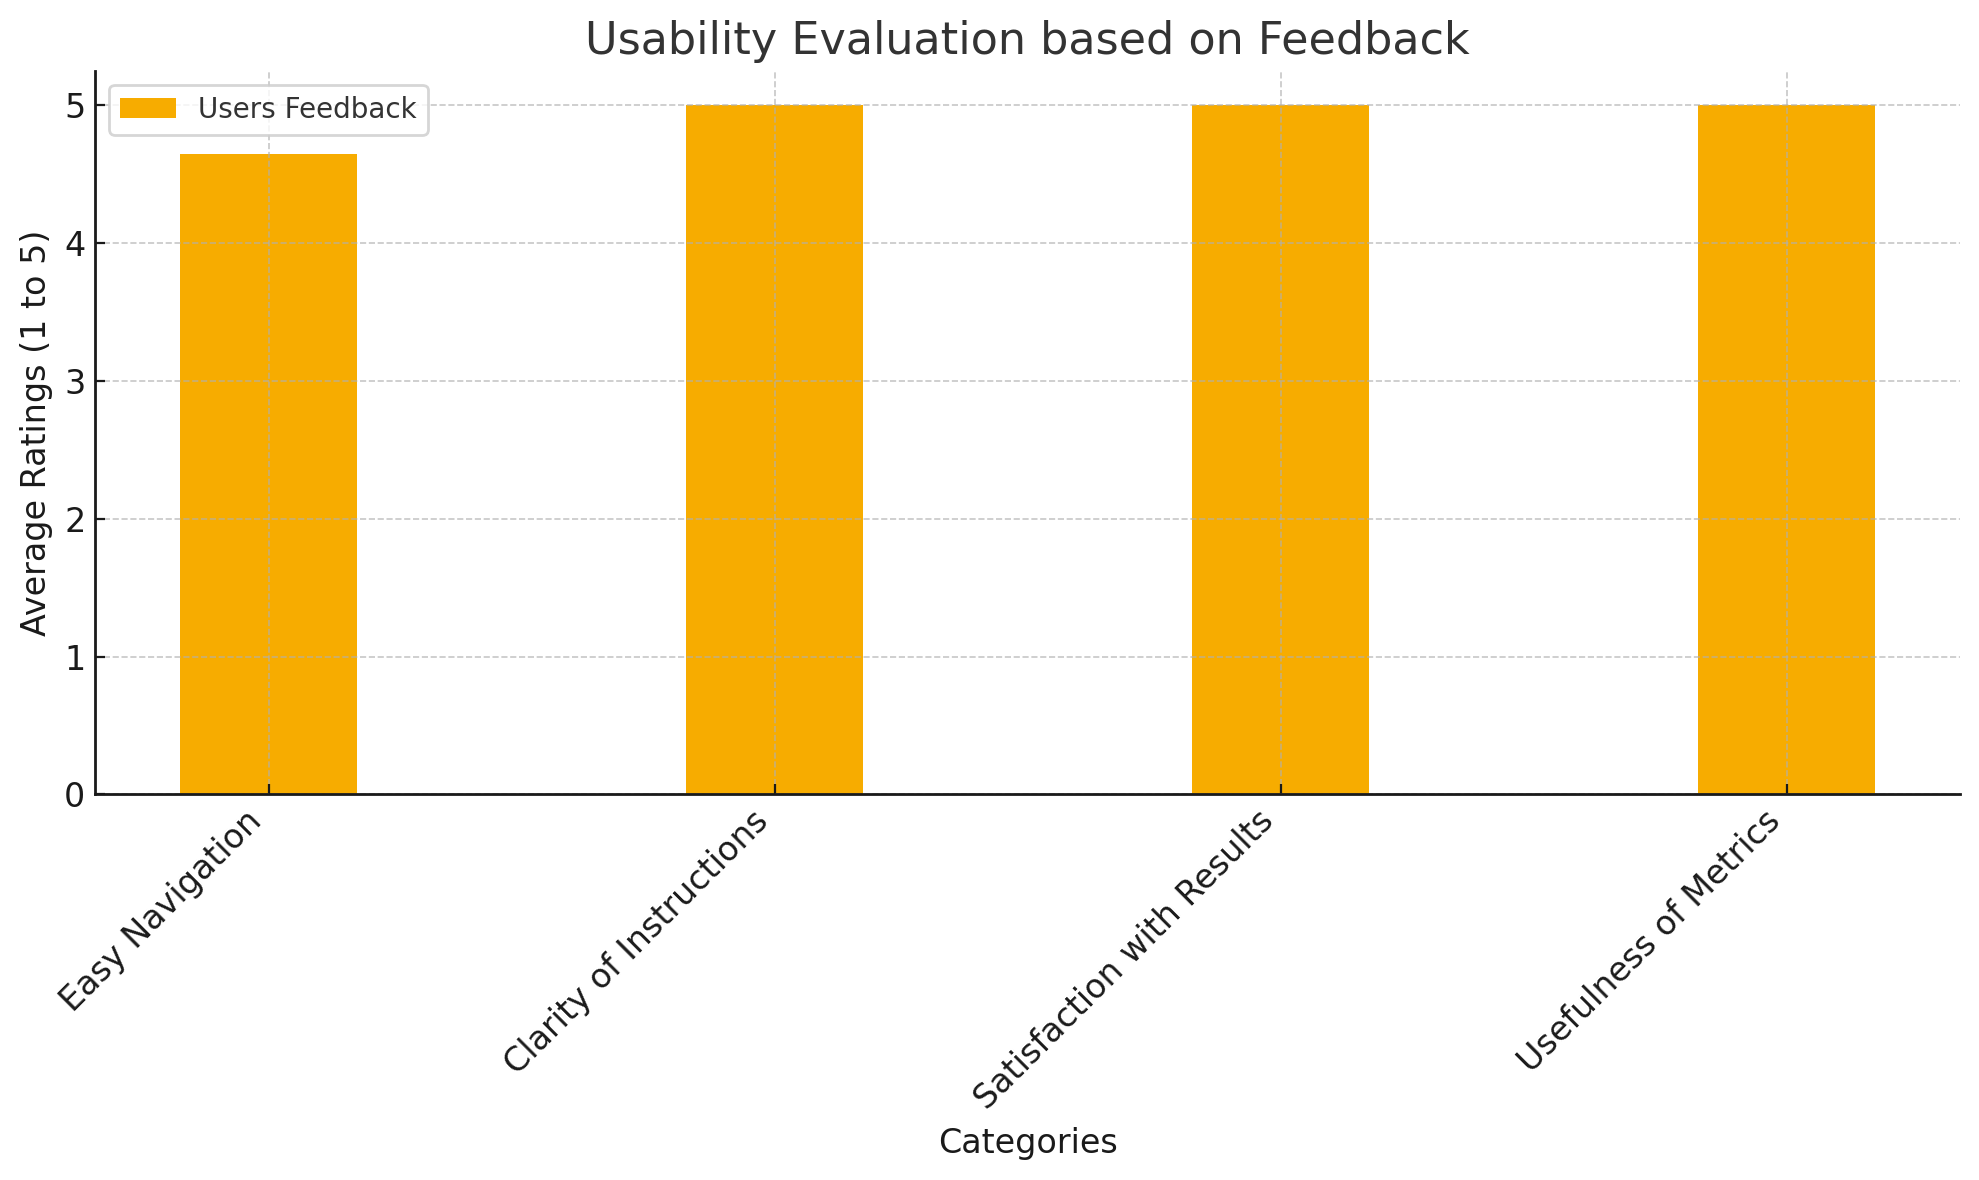
\includegraphics[width=0.6\textwidth]{figs/usability_grouped_bars.png} 
    \caption{Usability Evaluation: Ease of Navigation and Clarity of Instructions.}
    \label{fig:usability}
\end{figure}

Users rated both the ease of navigation and the clarity of instructions provided. As shown in Figure \ref{fig:usability}, both categories received high ratings, indicating that the software's interface was intuitive and well-designed.

Overall, the feedback was overwhelmingly positive. Most users reported a high level of satisfaction with the software's intuitive interface, with many describing it as "very intuitive" and "user-friendly." All respondents confirmed that they did not experience any difficulties navigating the software. Additionally, the explanations provided for the functionalities were considered clear by all users, indicating that the design and guidance within the software successfully facilitated a smooth user experience.

The analysis results themselves were deemed clear and comprehensible, with users unanimously agreeing that the software met or exceeded their expectations. Notably, the metrics provided by the software were highlighted as particularly useful for their work, suggesting that the software successfully addresses key analytical needs in genomic analysis. Users expressed a high likelihood of recommending the software to colleagues, demonstrating strong approval of its functionality and usefulness.

Suggestions for improvement were minimal, with a few users recommending performance enhancements and the inclusion of additional features, such as tailoring the software for \ac{cnvs} analysis. Nevertheless, users appreciated the versatility of the software, particularly the ability to zoom into specific regions and generate metrics for gene panels, genes, and exons.

The qualitative feedback collected highlights the most common positive aspects and suggested improvements. Overall, the feedback from the questionnaire indicates that the software is well-received, providing a user-friendly, intuitive, and efficient tool that meets the needs of various professionals in the genomic field. The overwhelmingly positive responses suggest that the software has significant potential for widespread adoption, with only minor adjustments needed to further enhance its performance and expand its capabilities.




